\documentclass[10pt,a4paper, titlepage]{article}
\usepackage{hyperref, parskip}
\usepackage[super,sort&compress,comma]{natbib}
\usepackage{graphicx}
\usepackage{mathtools}
\usepackage{amssymb}
\usepackage{chemformula}
\usepackage[section]{placeins}
\usepackage{float}
\title{Relevant papers for sodium-rich antiperovskite solid electrolytes}
\author{Benedek Goldmann}

\begin{document}

\maketitle
\tableofcontents
\clearpage

\part{Papers on Conductivity}

\section{Wang et al. (2015): Structural manipulation approaches towards enhanced sodium ionic conductivity in Na-rich antiperovskites}

\subsection{Methods}

\begin{itemize}
  \item Syntheis via grinding and annealing
  \item Powder X-ray diffraction
  \item Differential thermoanalyses between 323K and 623K
  \item DFT with CASTEP at GGA level with 2x2x2 supercell
\end{itemize}

\subsection{Synthesis and structure}

\begin{itemize}
  \item Made \ch{Na2O} fresh
  \item Synthesis via grinding and annealing
  \item \ch{Na3OI} difficult to synthesise due to \ch{Na4OI2} byproduct
  \item \ch{Na3OCl} lattice parameter: 4.4908 $\AA$
\end{itemize}

\subsection{Experimental conductivity}

\begin{figure}[H]
\centering
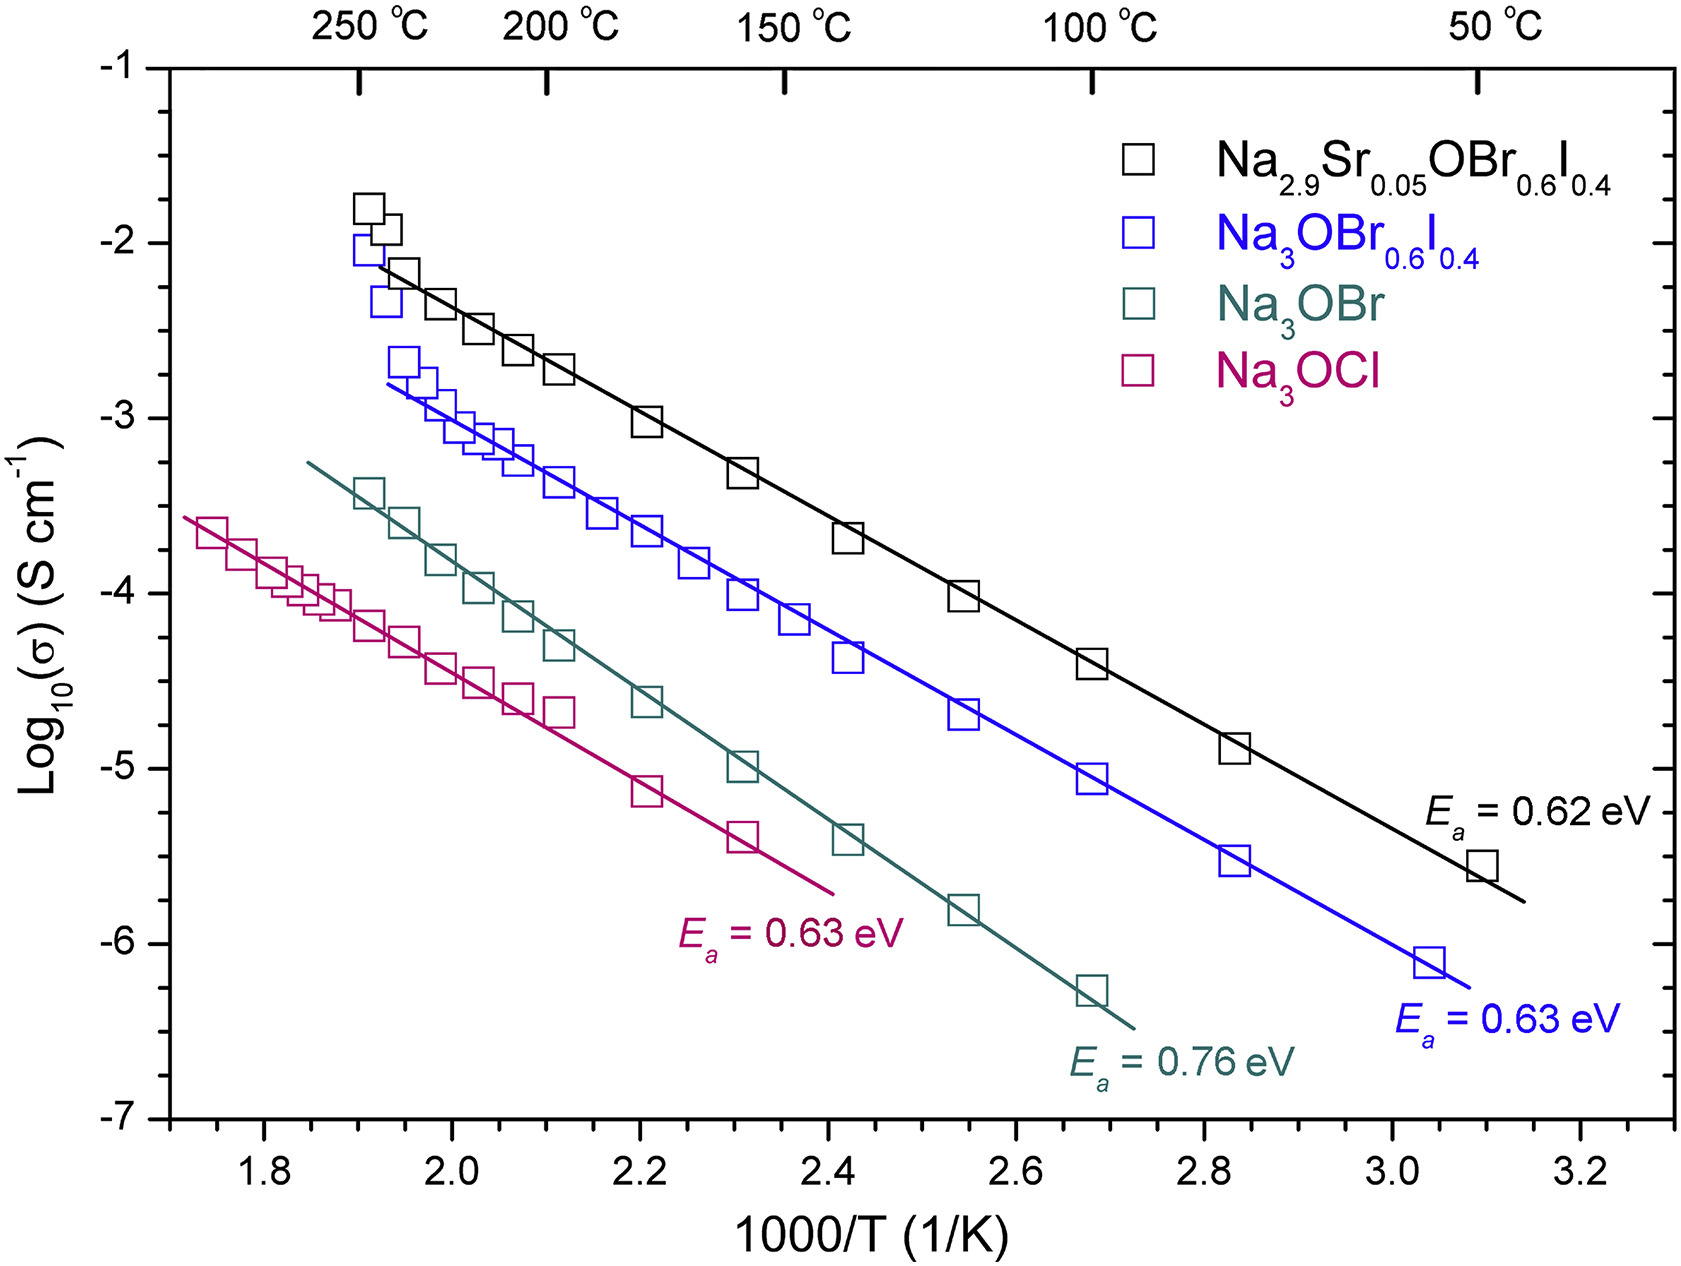
\includegraphics[width=7cm]{Wang2015_experimental.jpg}
\end{figure}

\subsection{Calculated conductivity}

\begin{figure}[H]
\centering
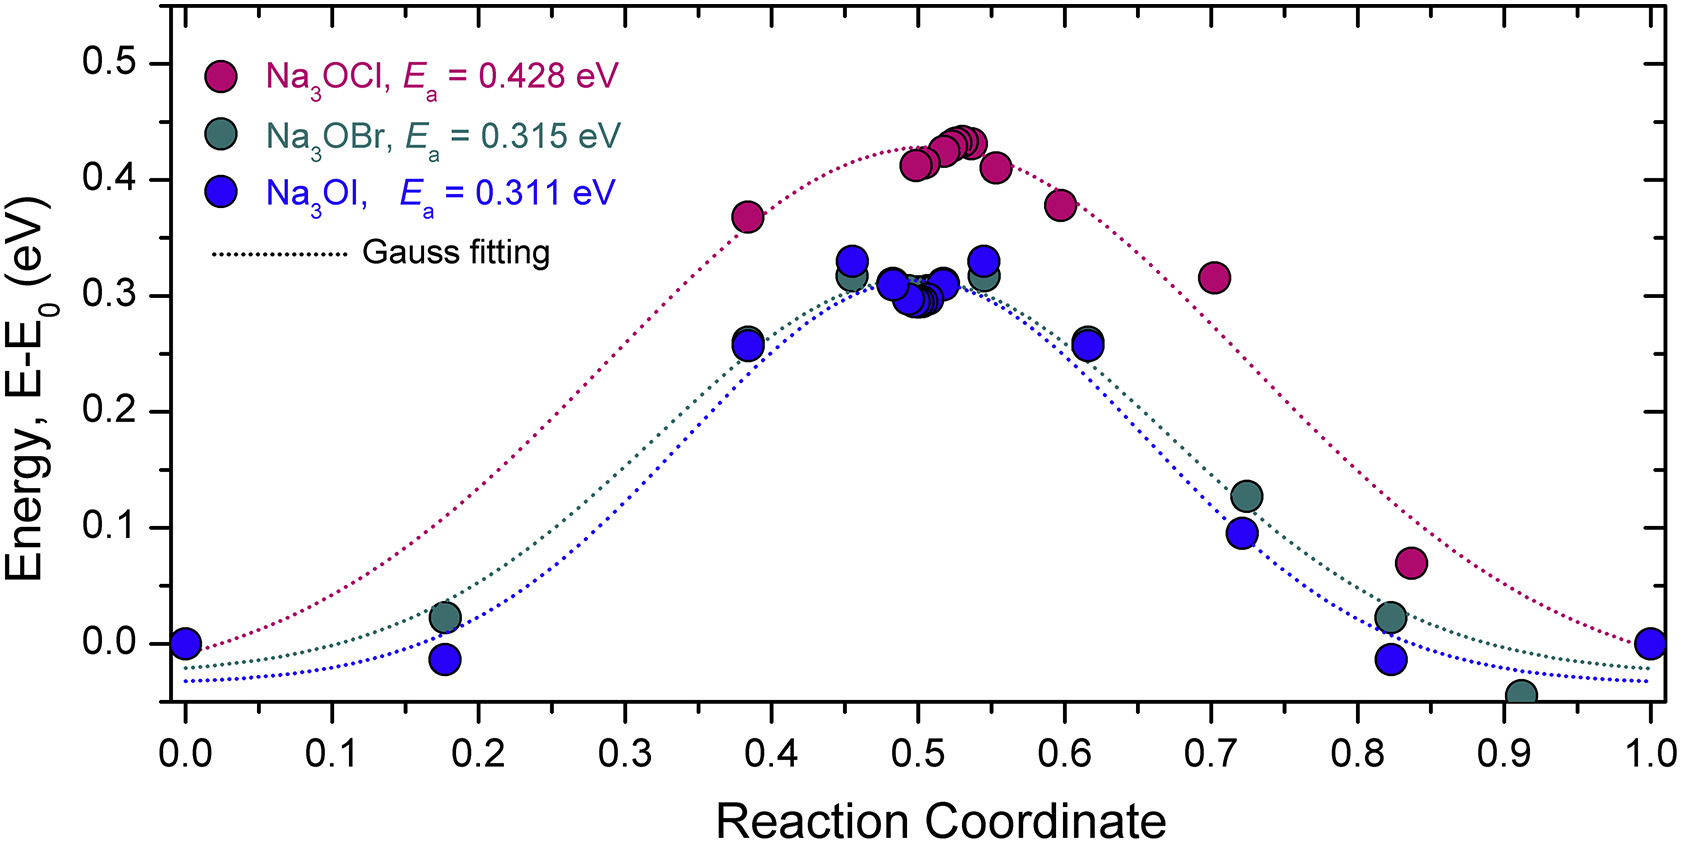
\includegraphics[width=7cm]{Wang2015_calculated.jpg}
\end{figure}

\subsection{Conclusion}

\begin{itemize}
  \item Great improvement in conductivity achievable via manipulation
  \item These include halogen-size-mismatch and alkali-earth doping
\end{itemize}

\section{Zhu et al. (2016): Sodium Ion Transport Mechanisms in Antiperovskite Electrolytes \ch{Na3OBr} and \ch{Na4OI2}: An in Situ Neutron Diffraction Study}

\subsection{Methods}

\begin{itemize}
  \item Synthesis via solid-state raction and sintering with freshly made \ch{Na2O}
  \item Neutron powder diffraction
  \item Impedance spectroscopy
  \item DFT with CASTEP and generalised gradient approximation (GGA) with 2x2x2 supercell fo \ch{Na3OBr} and 2x2x1 supercell for \ch{Na4OI2}
\end{itemize}

\subsection{Synthesis and structure}

\begin{itemize}
  \item \ch{Na3OBr} is antiperovskite, \ch{Na4OI2} is a type of antiperovskite, where antiperovskite and rocksalt layers change alternate
  \item This means 3D migration for \ch{Na3OBr}, but 2D for \ch{Na4OI2}
  \item\ch{Na4OI2} has higher concentration of Na vacancies
\end{itemize}

\subsection{Experimental conductivity}

\begin{figure}[H]
\centering
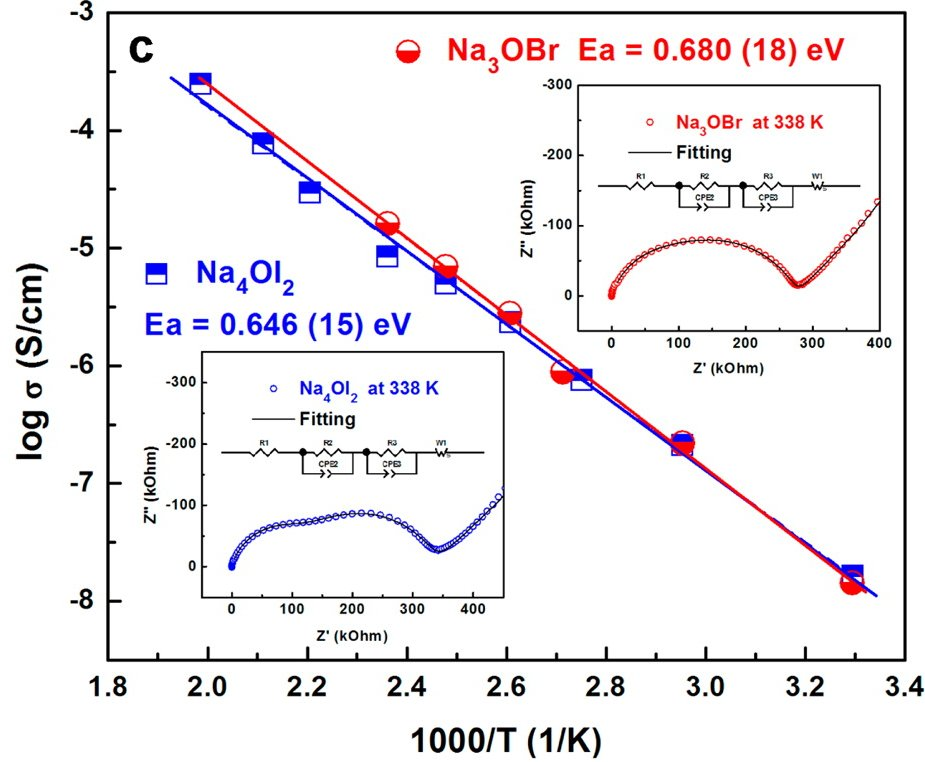
\includegraphics[width=7cm]{Zhu_conductivity.jpeg}
\end{figure}

\subsection{Calculated conductivity}

\begin{figure}[H]
\centering
\includegraphics[width=7cm]{ZHu_calculated.jpeg}
\end{figure}

\subsection{Conclusions}

\begin{itemize}
  \item the main sodium transport pathway in both cubic \ch{Na3OBr} and layered \ch{Na4OI2} is between the nearest \ch{Na+} ions in the \ch{NaO6} octahedra building block of the antiperovskite
\end{itemize}

\section{Nguyen et al. (2016): Experimental and Computational Evaluation of a Sodium-Rich
Anti-Perovskite for Solid State Electrolytes}

\subsection{Methods}

\begin{itemize}
  \item Synthesis via solid-state reaction (from pre-made \ch{Na2O} then either cold pressing or spark plasma sintering (SPS)
  \item Scanning electron microscopy
  \item X-ray diffraction
  \item Electrochemical impedance spectroscopy
  \item Defect calculations from DFT via VASP with prrojector-augmented wave (PAW) method with GGA on a 3x3x3 supercell
\end{itemize}

\subsection{Synthesis and structure}

\begin{itemize}
  \item Both cold pressing and SPS resulted in antiperovskite \ch{Na3OBr}
  \item Lower porosity for SPS sample as well as higher density
\end{itemize}

\subsection{Defects}

\begin{figure}[H]
\centering
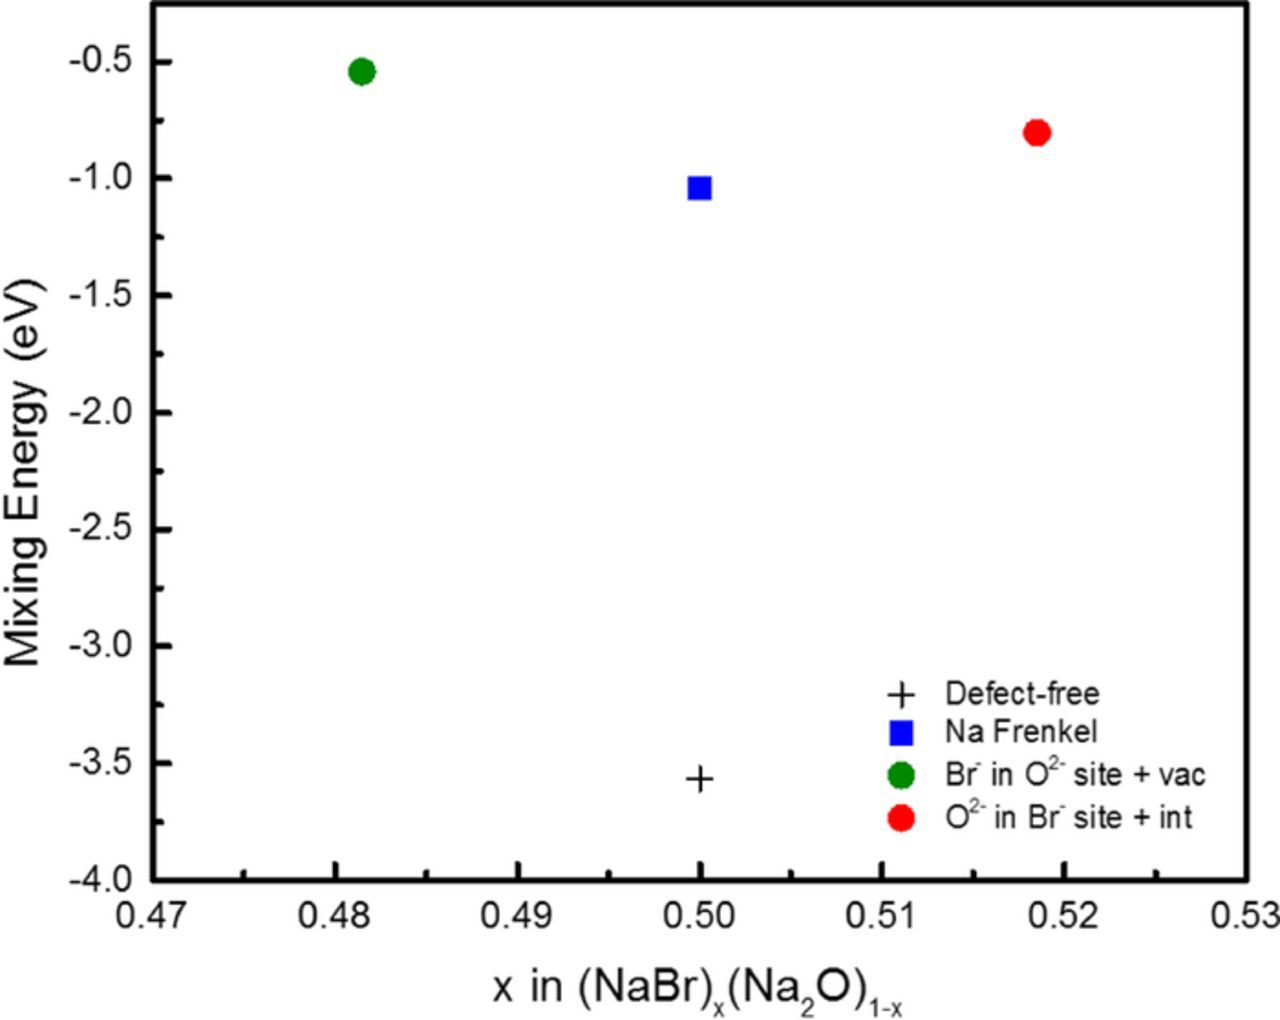
\includegraphics[width=7cm]{Nguyen2016_defects.jpeg}
\end{figure}

\subsection{Experimental conductivity}

\begin{figure}[H]
\centering
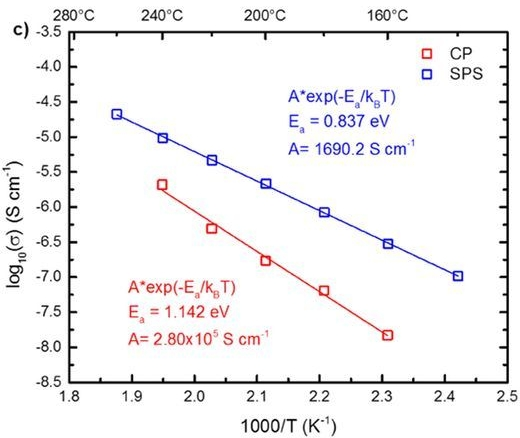
\includegraphics[width=7cm]{Nguyen2016_experimental.jpeg}
\end{figure}

\subsection{Conclusions}

\begin{itemize}
  \item SPS is a successful method for synthesis of less porous antiperovskites with higher conductivities
  \item Defects are too high in energy to be induced thermally, so alio- and isovalent doping necessary in \ch{Na3OBr}
\end{itemize}

\section{Wan et al. (2018): A first principle study of the phase stability, ion transport and substitution strategy for highly ionic conductive sodium antipervoskite as solid electrolyte for sodium ion batteries}

\subsection{Methods}

\begin{itemize}
  \item Used VASP code to run DFT calculations with the projector augmented wave (PAW) method and generalised gradient approximation (GGA)
  \item Defect energies and NEB migrations on 3x3x3 supercell (135 atoms)
  \item AIMD calculations on 2x2x2 supercell, 100ps in length and with 2fs time-steps between 800 and 1500K
\end{itemize}

\subsection{Structure}

\begin{itemize}
  \item \ch{Na3OCl} lattice parameter: 4.54 $\AA$
  \item Band gap: 2.0 eV
  \item Formation energy: -72.7 meV/formula unit
\end{itemize}

\subsection{Defects and doping}

\begin{itemize}
  \item Used 3 possible configuration for defect energies
  \item NaCl Schottky lowest energy
  \item Alkaline earth solution energy decreases across group (used oxide substitution)
  \item Binding energy lowest for Ca and Sr
\end{itemize}

\subsection{Conductivity}

\begin{itemize}
  \item Found vacancy hop migration energy to be 0.61 eV
  \item Concluded that the migration barrier is least increased by Ca (0.66 eV)
\end{itemize}

\begin{figure}[H]
\centering
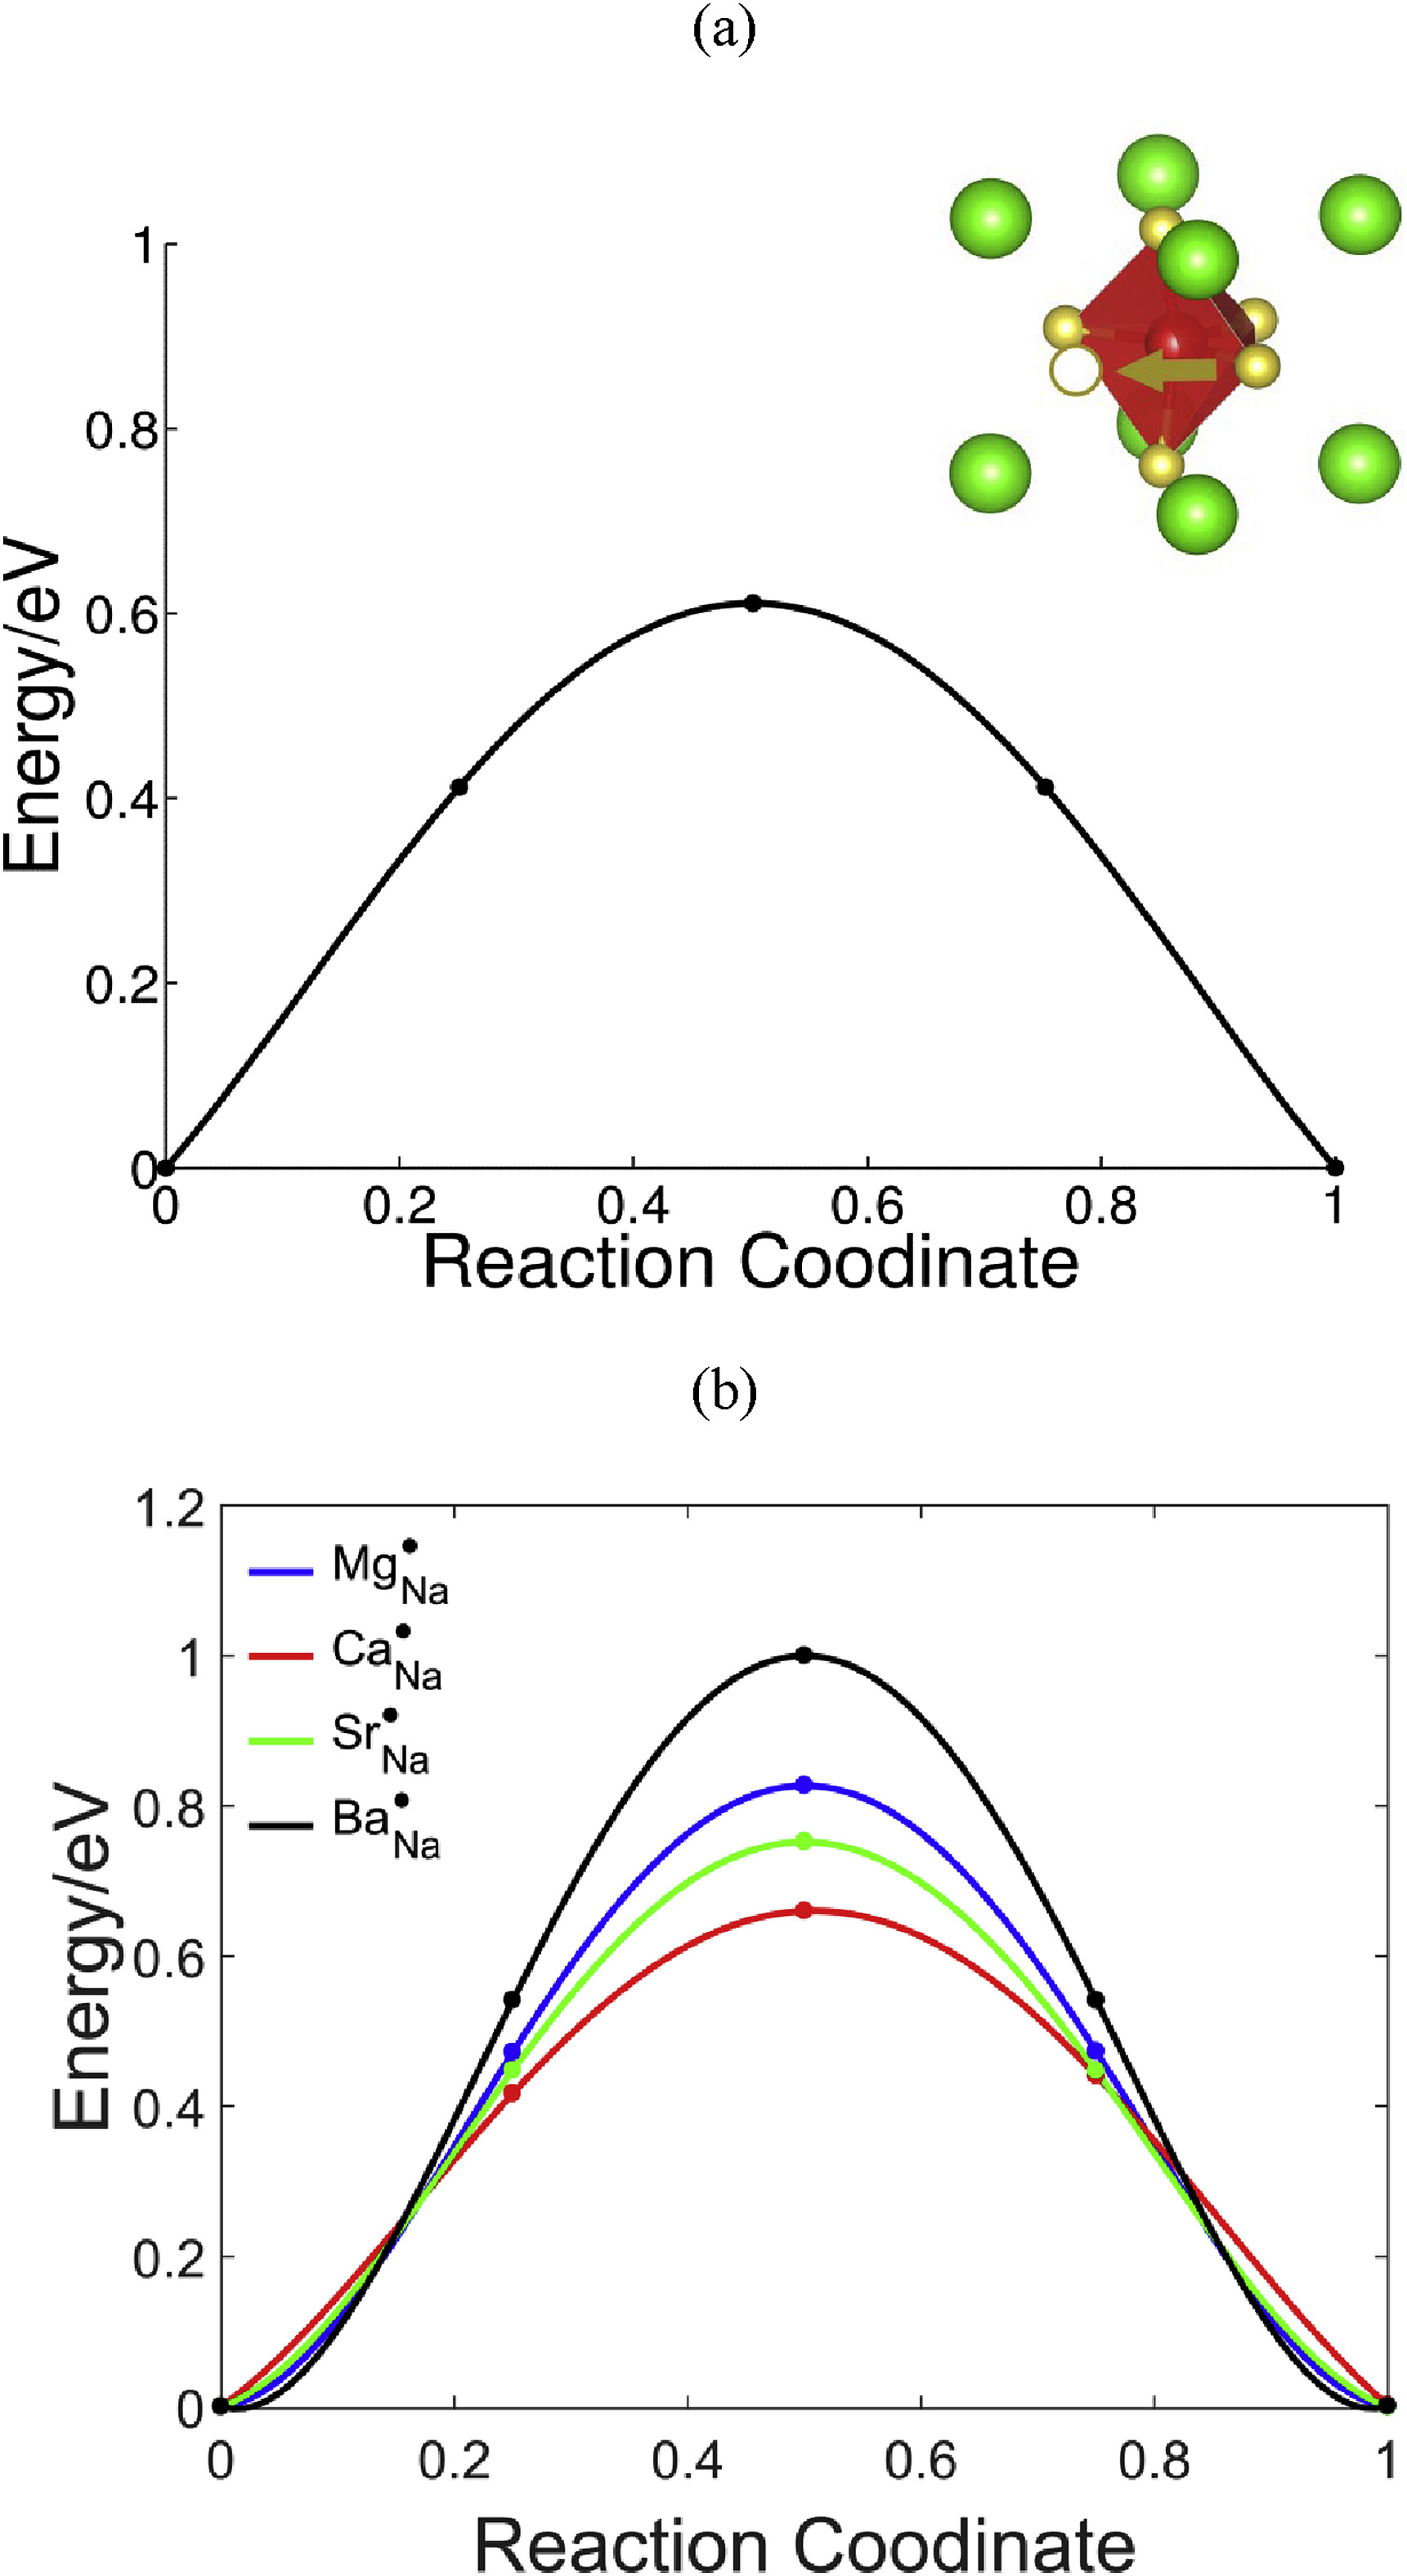
\includegraphics[width=7cm]{Wan2018_DFT.jpg}
\end{figure}

\begin{itemize}
  \item Ran AIMD on \ch{Na_{2.875}OCl} and \ch{Na_{2.75}Ca_{0.125}OCl} and found activation energies of 0.42 eV,  and 0.47 eV, respectively
  \item AIMD also found extrapolated conductivities at 300K of 3.92-8.19 $\mu$S/cm and 0.53-4.41 $\mu$S/cm, respectively
\end{itemize}

\begin{figure}[H]
\centering
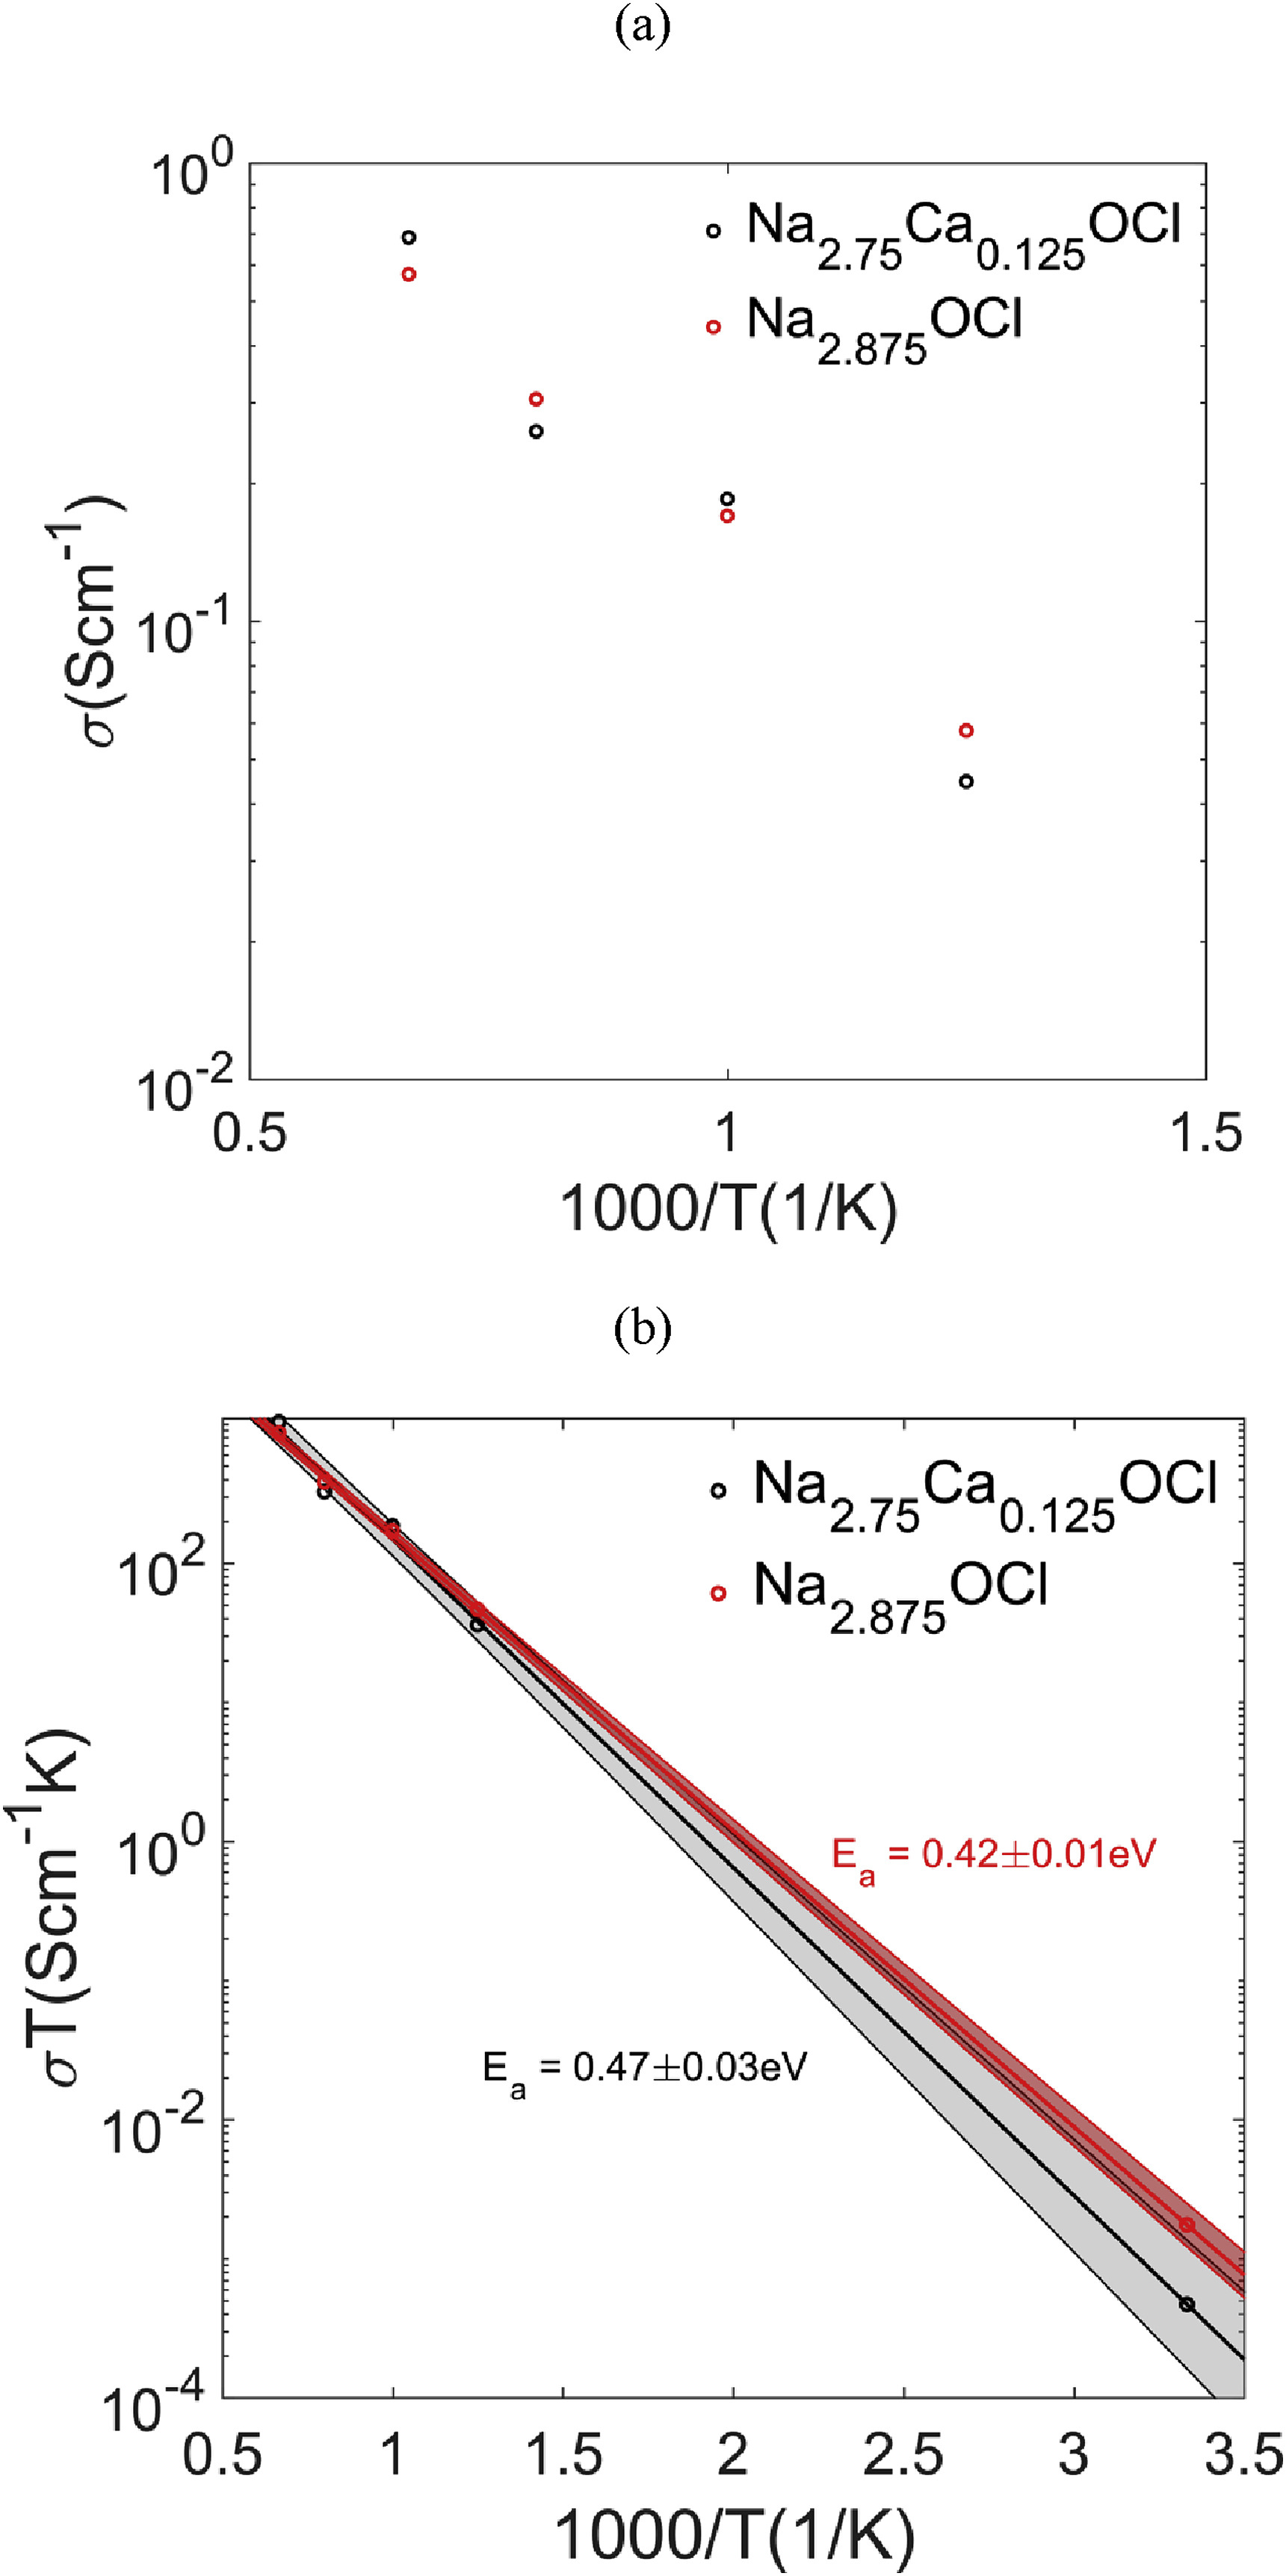
\includegraphics[width=7cm]{Wan2018_AIMD.jpg}
\end{figure}

\subsection{Conclusions}

\begin{itemize}
  \item NaCl Schottky favoured, so vacancy hopping likely
  \item Ca most promissing as cation dopant
\end{itemize}

\section{Yu et al. (2018): Theoretical design of double anti-perovskite \ch{Na6SOI2} as a super-fast ion conductor for solid \ch{Na+} ion batteries}

\subsection{Methods}

\begin{itemize}
  \item DFT via VASP with PAW method and GGA
  \item AIMD runs with 10 ps equilibration, followed by 80 ps runs with 2 fs steps at temperature range 600-1200 K
\end{itemize}

\subsection{Defects}

\begin{figure}[H]
\centering
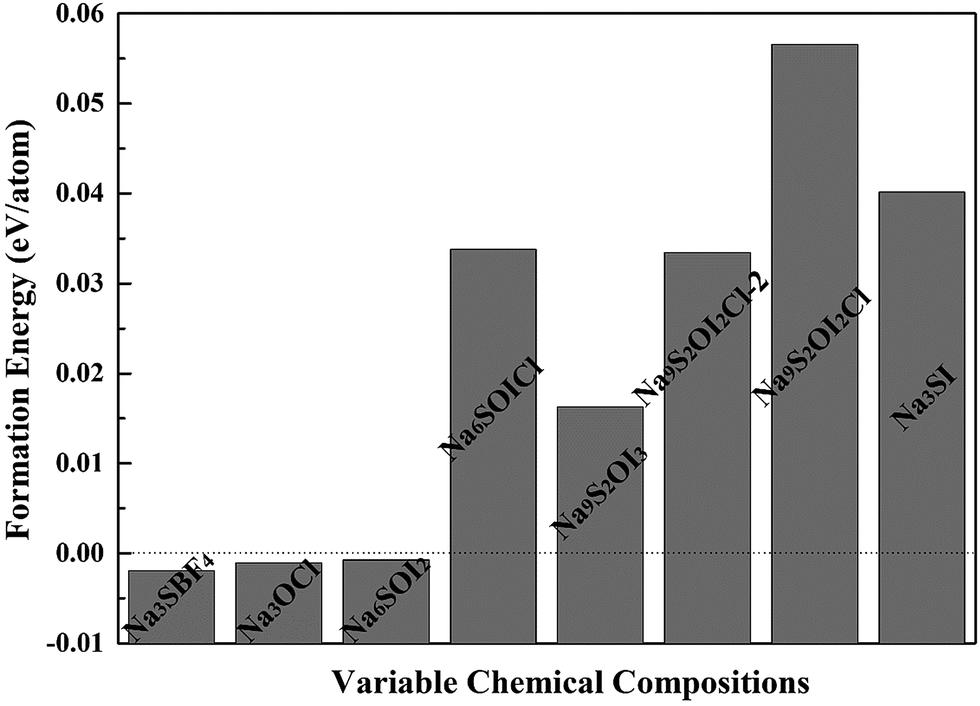
\includegraphics[width=7cm]{Yu2018_defects.jpeg}
\end{figure}

\subsection{Calculated conductivity}

\begin{figure}[H]
\centering
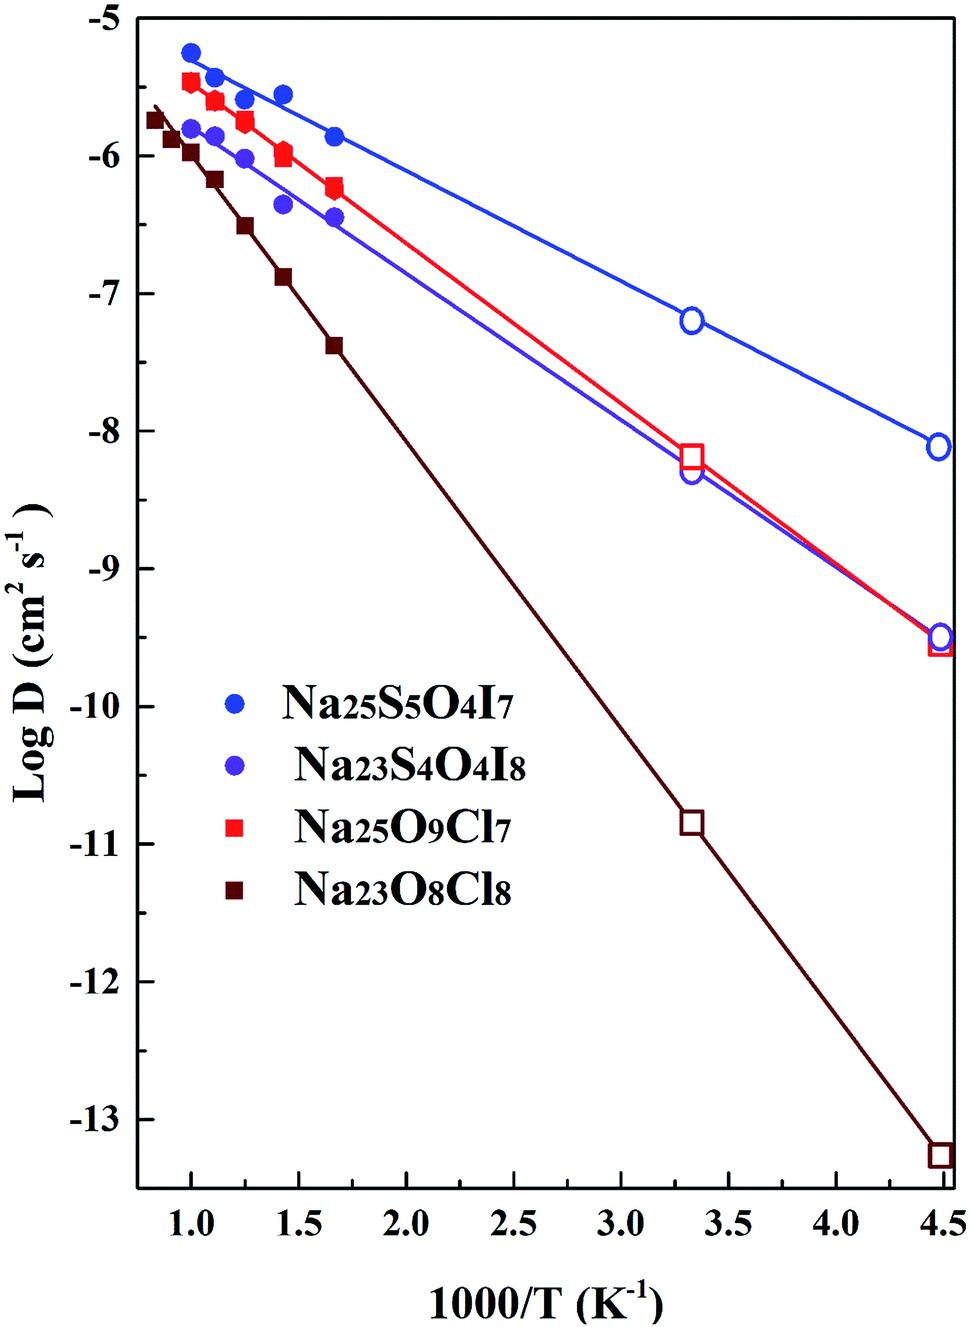
\includegraphics[width=7cm]{Yu2018_conductivity.jpeg}
\end{figure}

\subsection{Conclusions}

\begin{itemize}
  \item Moderate off-stoichiometric compositional deviation in the double-anti-perovskite phase leads to significant reduction of the activation barrier for Na+ transportation
  \item Very low activation energy of about 0.16 eV for \ch{Na25S5O4I7}
\end{itemize}

\section{Dawson et al. (2018): Composition Screening of Lithium- and Sodium-Rich Anti-Perovskites for Fast-Conducting Solid Electrolytes}

\subsection{Methods}

\begin{itemize}
  \item GULP code with the Mott-Littleton approximation for defect calculations
  \item LAMMPS code for MD calculations
  \item MD calculations on supercell with about 5000 ions, 10ns in length with 2fs timesteps in temperature range 500K-1000K
\end{itemize}

\subsection{Structure}

\begin{itemize}
  \item \ch{Na3OCl} lattice parameter: 4.501 $\AA$
\end{itemize}

\subsection{Defects}

\begin{figure}[H]
\centering
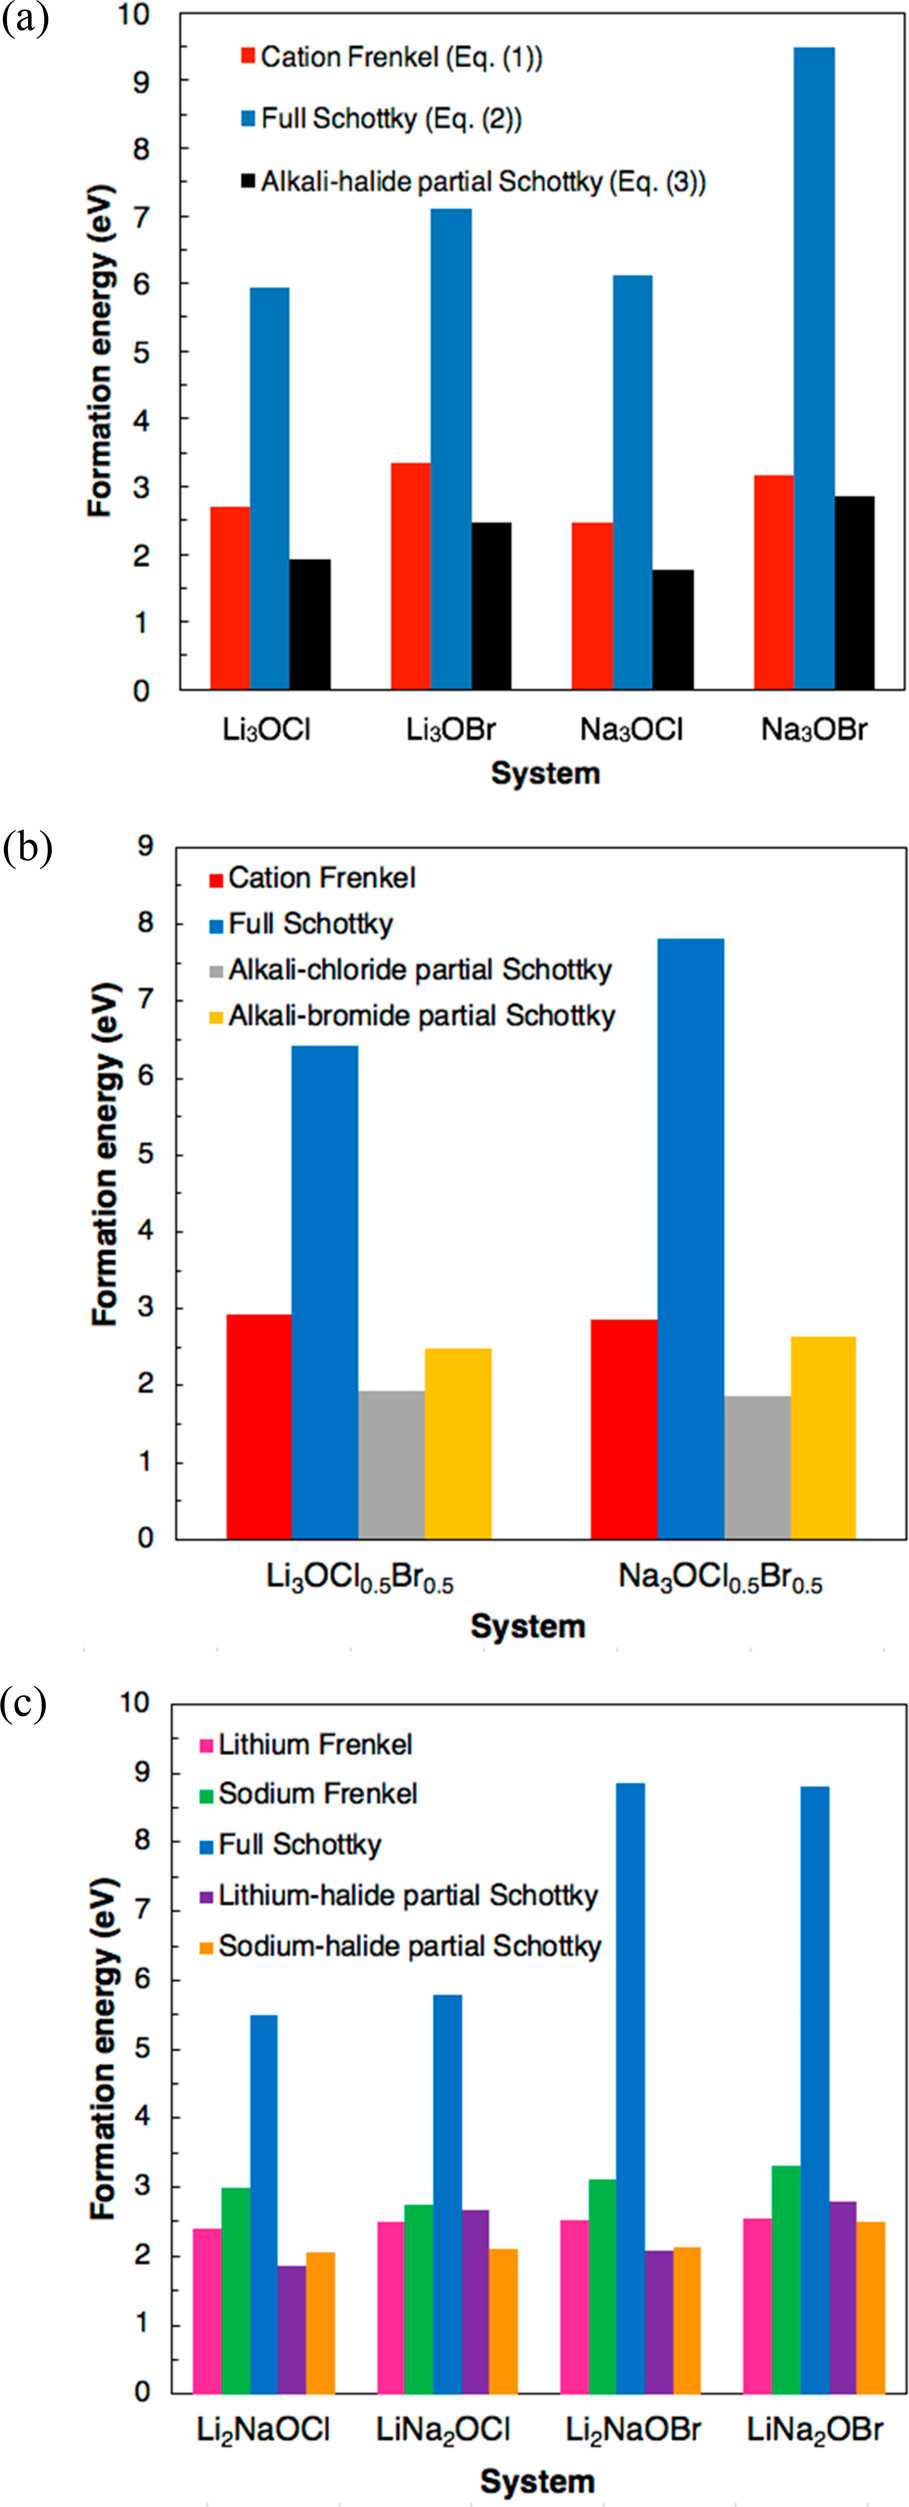
\includegraphics[width=7cm]{Dawson2018_defects.jpeg}
\end{figure}

\subsection{Conductivity}

\begin{itemize}
  \item \ch{Na3OCl} has slightly higher activation energy than \ch{Na3OBr}
  \item \ch{Na3OCl_{0.5}Br_{0.5}} can lower activation energy further
\end{itemize}

\begin{figure}[H]
\centering
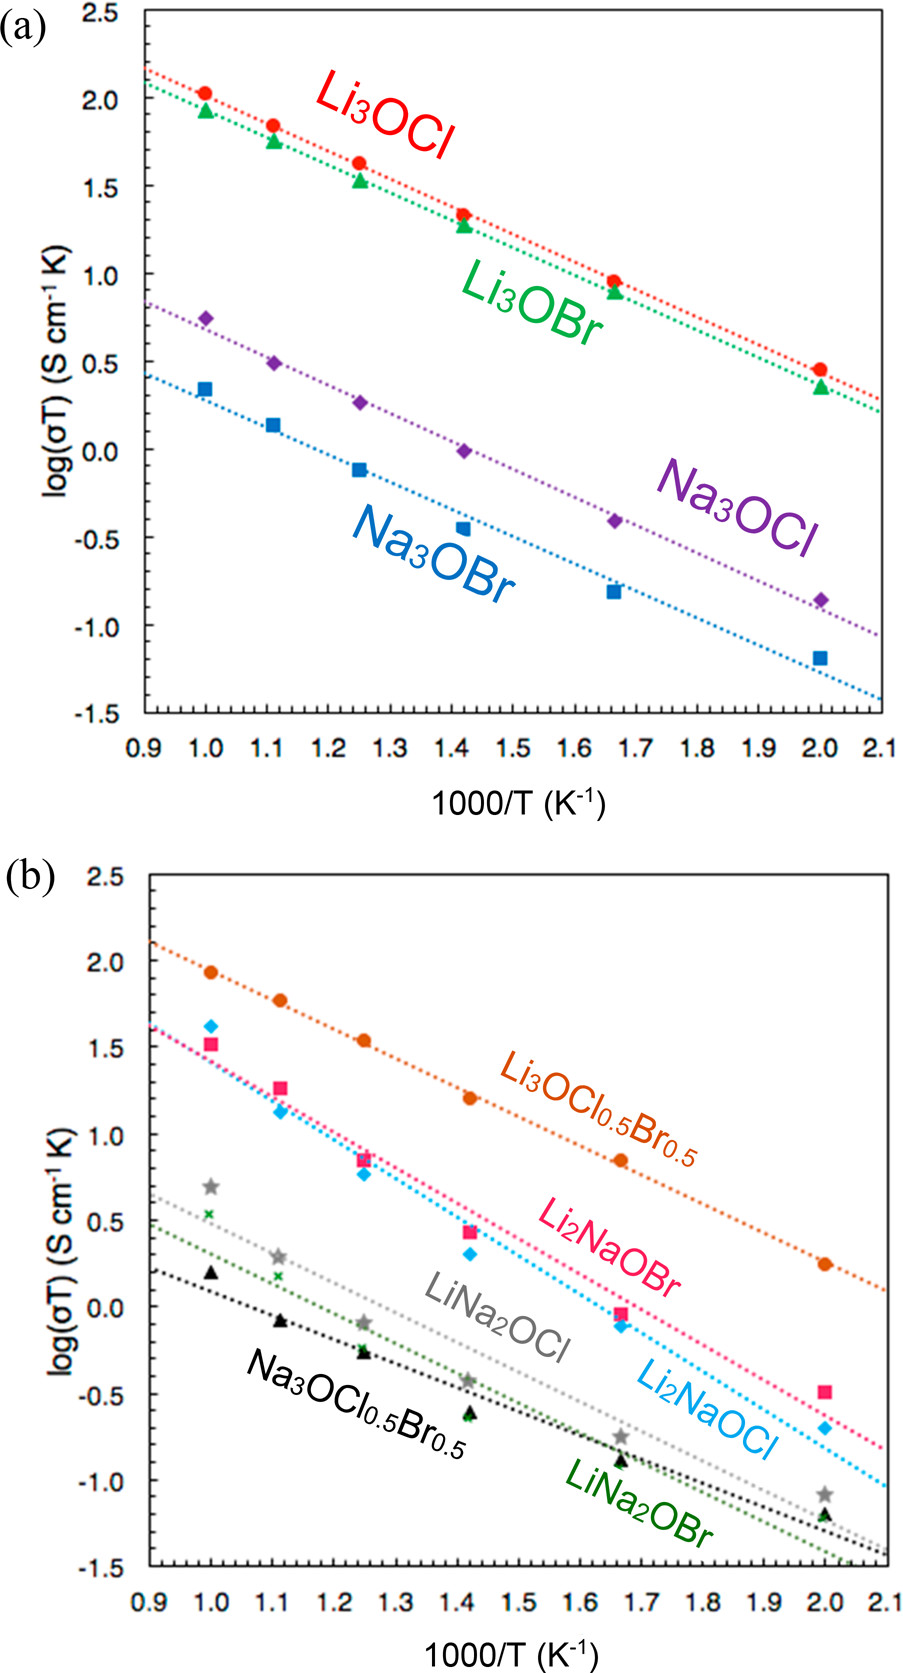
\includegraphics[width=7cm]{Dawson2018_conductivity.jpeg}
\end{figure}

\subsection{Conclusions}

\begin{itemize}
  \item Alkali-halide partial Schottky dominant
  \item Halide-ion mixing does not significantly improve conductivity
  \item Activation energy barrier high for mixed alkali systems
\end{itemize}

\section{Sun et al. (2019): Rotational Cluster Anion Enabling Superionic Conductivity in
Sodium-Rich Antiperovskite \ch{Na3OBH4}}

\subsection{Methods}

\begin{itemize}
  \item Synthesis via solid-state reaction of \ch{Na2O} and \ch{NaBH4}
  \item Neutron powder diffraction
  \item X-ray powder diffraction
  \item Differential scanning calorimetry
  \item $^{23}$Na NMR
  \item AIMD with 10ps equilibration and 40ps of simulation
\end{itemize}

\subsection{Synthesis and structure}

\begin{itemize}
  \item Synthesis of sulfide alternatives failed (possibly due to the tolerance factor
  \item Small tetragonal and orthorombic distortion from cubic in \ch{Na3OBH4} 
  \item Two Na sites in NMR of \ch{Na3OBr}
\end{itemize}

\subsection{Conductivity}

\begin{itemize}
  \item Cold-pressed pellet had low conductivity (maybe grain-boundary effect), so hot-pressed was used
\end{itemize}

\begin{figure}[H]
\centering
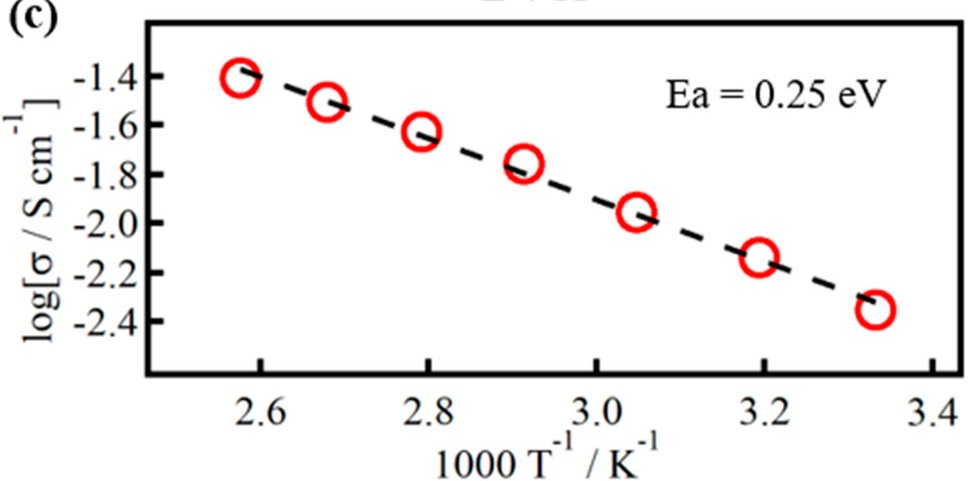
\includegraphics[width=7cm]{Sun2019_conductivity.jpeg}
\end{figure}

\subsection{Conclusions}

\begin{itemize}
  \item Rotation of \ch{BH4} group could be the cause of increased conductivity
\end{itemize}

\section{Yu et al. (2019): Theoretical tuning of Ruddlesden–Popper type anti-perovskite phases as superb ion conductors and cathodes for solid sodium ion batteries}

\subsection{Methods}

\begin{itemize}
  \item DFT via VASP with the projector augmented wave (PAW) method
  \item AIMD with 10 ps equilibrium, followed by 80ps of simulation with 2 fs steps at 900-1300 K
\end{itemize}

\subsection{Doping}

\begin{itemize}
  \item Numeral represents space group of the substituted species
\end{itemize}

\begin{figure}[H]
\centering
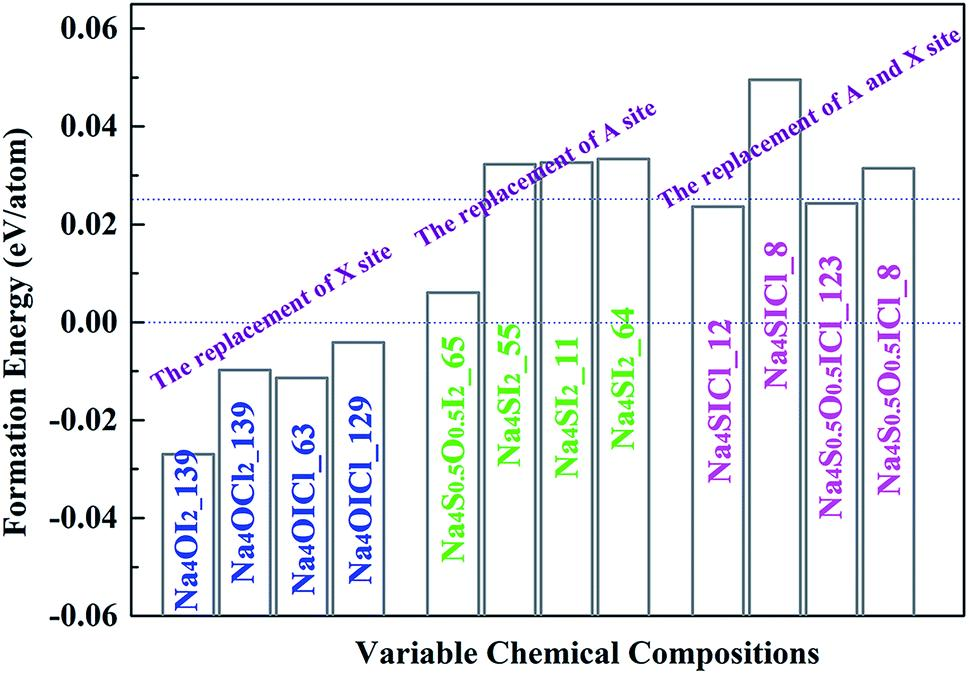
\includegraphics[width=7cm]{Yu2019_defects.jpeg}
\end{figure}

\subsection{Calculated conductivity}

\begin{figure}[H]
\centering
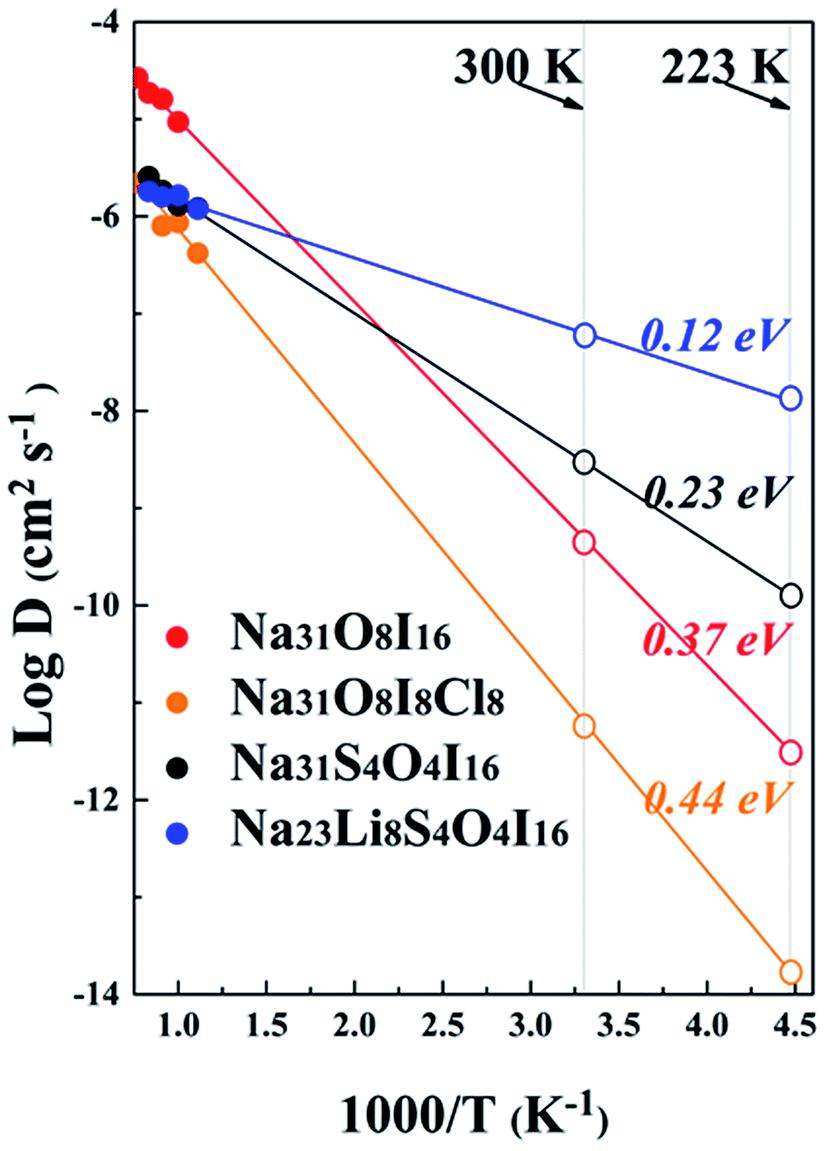
\includegraphics[width=7cm]{Yu2019_conductivity.jpeg}
\end{figure}

\subsection{Conclusions}

\begin{itemize}
  \item Discovery of a superb solid electrolyte \ch{Na3Lis_{0.5}O_{0.5}I2}, which exerts extremely low activation energy for \ch{Na+} diffusion, thus permitting a room temperature \ch{Na+} conductivity of over $6.3 \, mS \, cm^{-1}$
\end{itemize}

\section{Fang et al. (2019): Sodium Superionic Conductors Based on Clusters}

\subsection{Methods}

\begin{itemize}
  \item DFT via VASP with PAW and GGA
  \item AIMD with 40ps equilibrium, followed by 250ps simulation with 2 fs steps on 2x2x2 supercell
\end{itemize}

\subsection{Conductivity}

\begin{itemize}
  \item Migration profile for \ch{Na3S(BCl4)} at lower temperature (staggered line) and at higher temperature (solid line)
\end{itemize}

\begin{figure}[H]
\centering
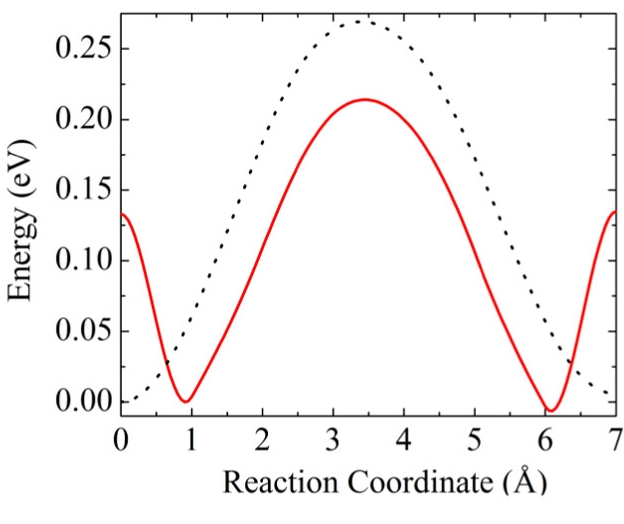
\includegraphics[width=7cm]{Fang2019_activation.jpeg}
\end{figure}

\begin{figure}[H]
\centering
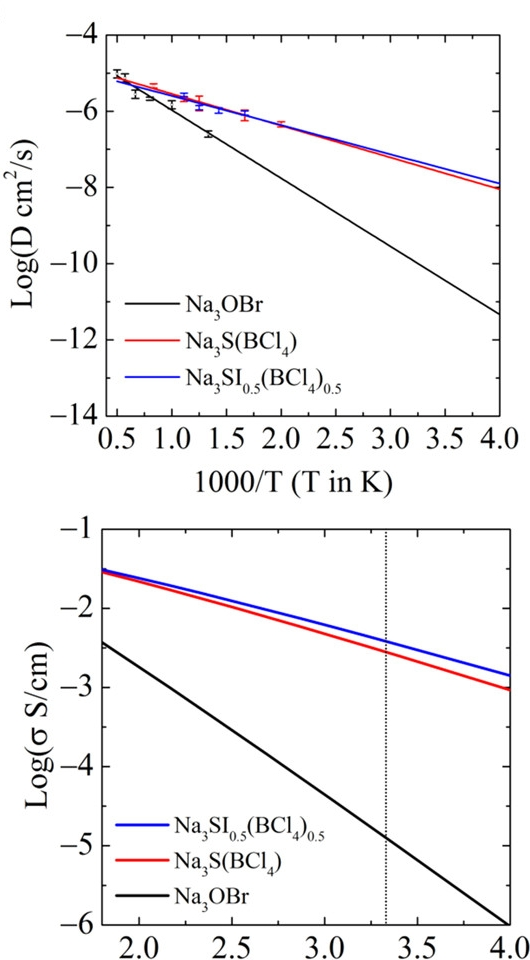
\includegraphics[width=7cm]{Fang2019_conductivity.jpeg}
\end{figure}

\subsection{Conclusions}

\begin{itemize}
  \item Clustered ions can enhance conductivity by creating a larger lattice
  \item Structures with both clustered and elementary ion can have even higher conductivities
\end{itemize}

\section{Ahiavi el at. (2020): Mechanochemical synthesis and ion transport properties of \ch{Na3OX} (X = Cl, Br, I and \ch{BH4}) antiperovskite solid electrolytes}

\subsection{Methods}

\begin{itemize}
  \item Synthesis via ball willing with and without annealing
  \item X-ray powder diffraction
  \item Impedance spectroscopy between 298 K and 373 K
  \item Thermal analysis
  \item Vibrational spectroscopy
  \item AIMD calculations via VASP code with projector augmented wave (PAW) method on 3x3x3 supercell at 600K, 800K and 1000K
\end{itemize}

\subsection{Synthesis and structure}

\begin{itemize}
  \item Made \ch{Na2O} fresh
  \item Synthesis via ball willing with and without annealing
  \item Sulfides could not be synthesised (unless with low sulfide content)
  \item \ch{Na3OCl} lattice parameter: 4.504 $\AA$
\end{itemize}

\subsection{Experimental conductivity}

\begin{figure}[H]
\centering
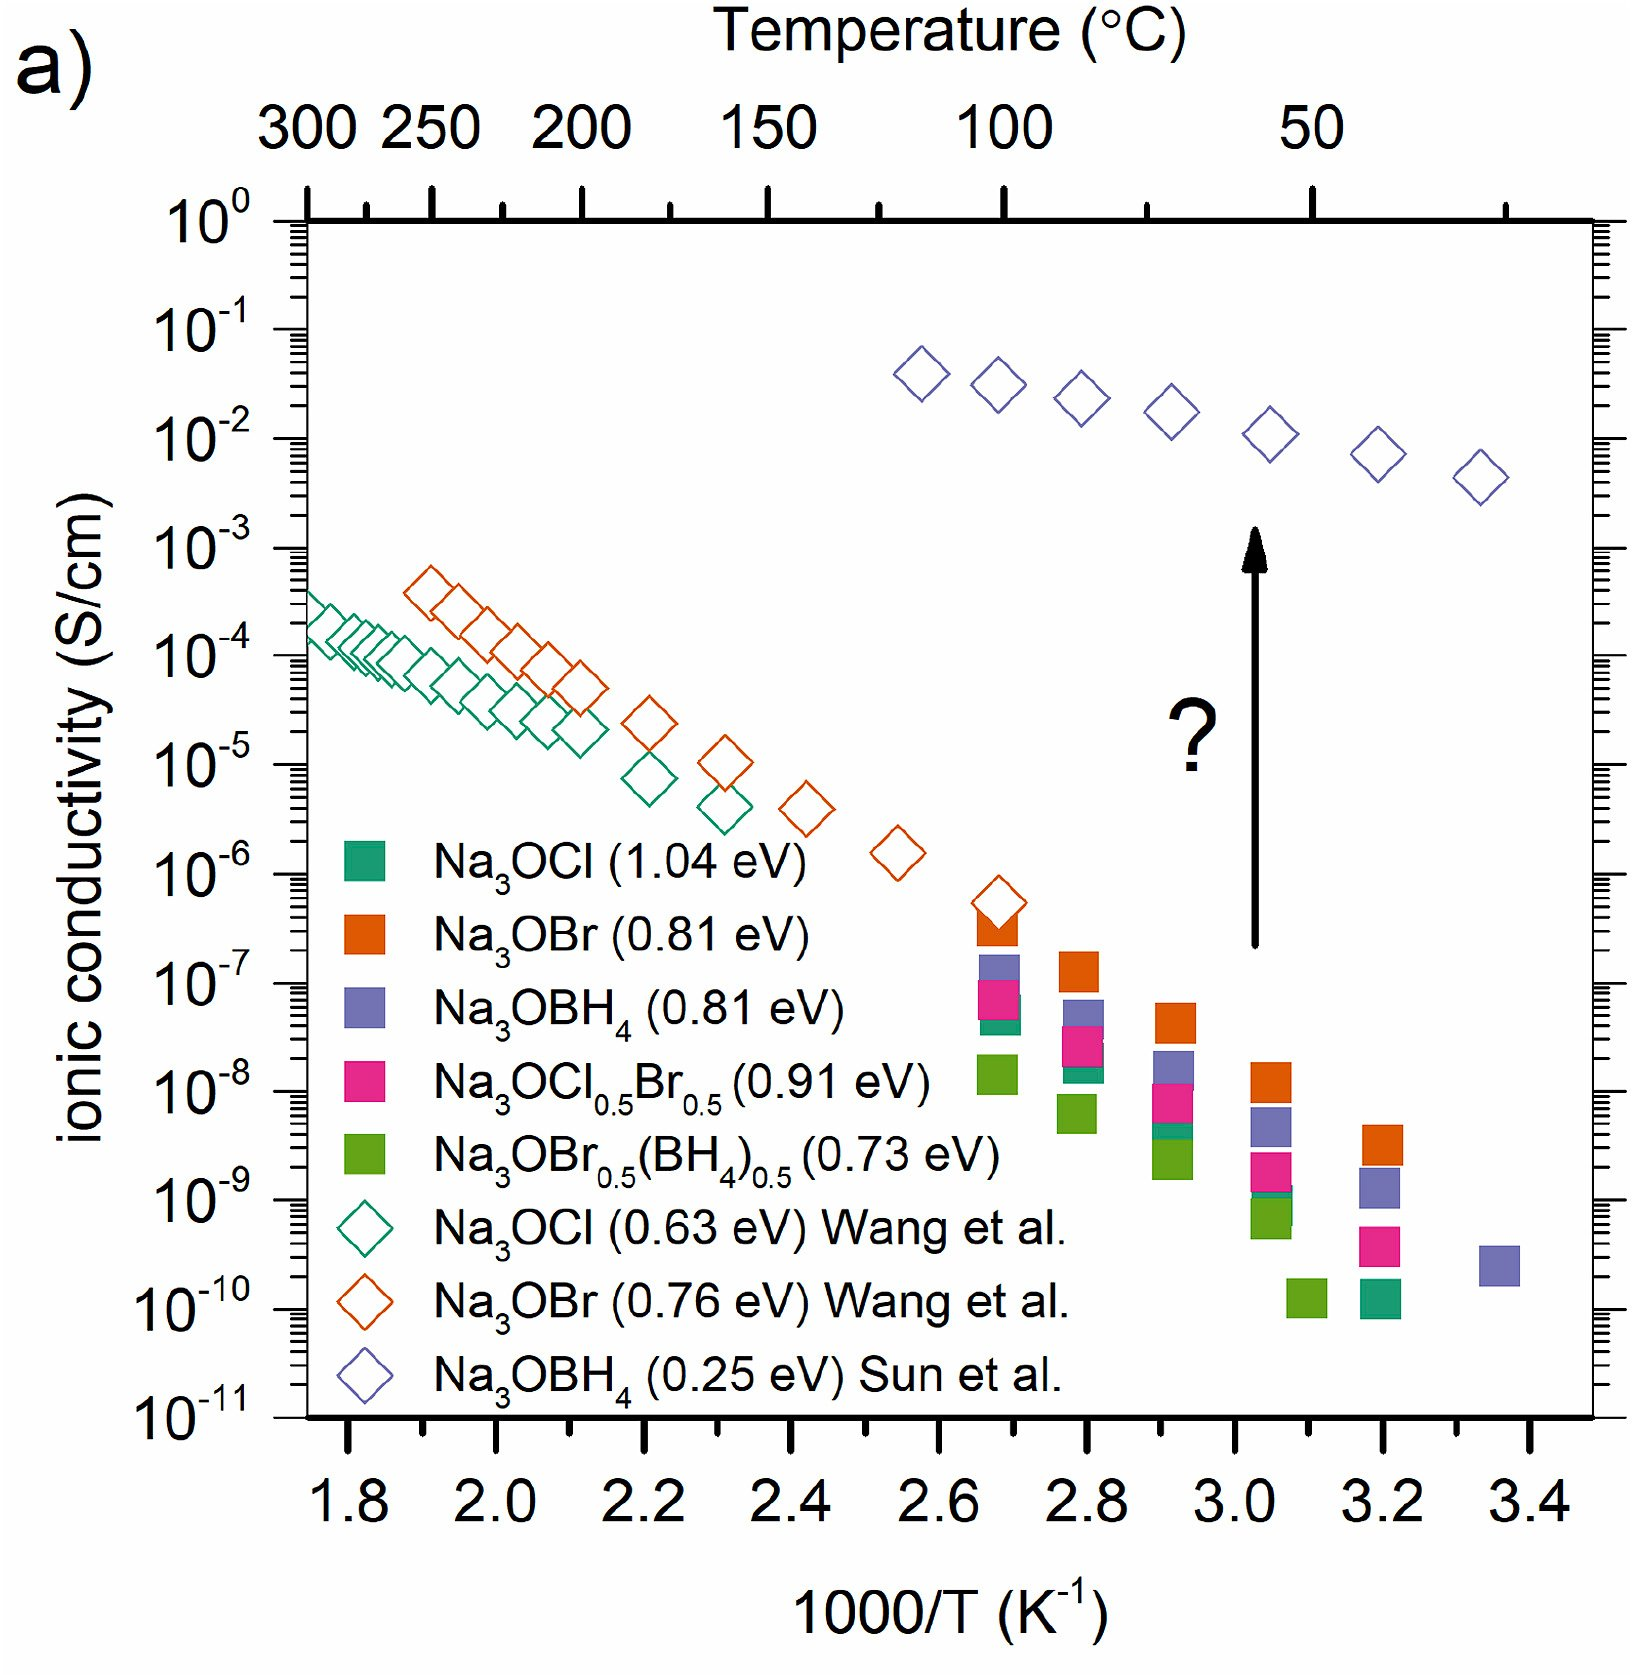
\includegraphics[width=7cm]{Ahiavi2020_experimental.jpg}
\end{figure}

\subsection{Calculated conductivity}

\begin{figure}[H]
\centering
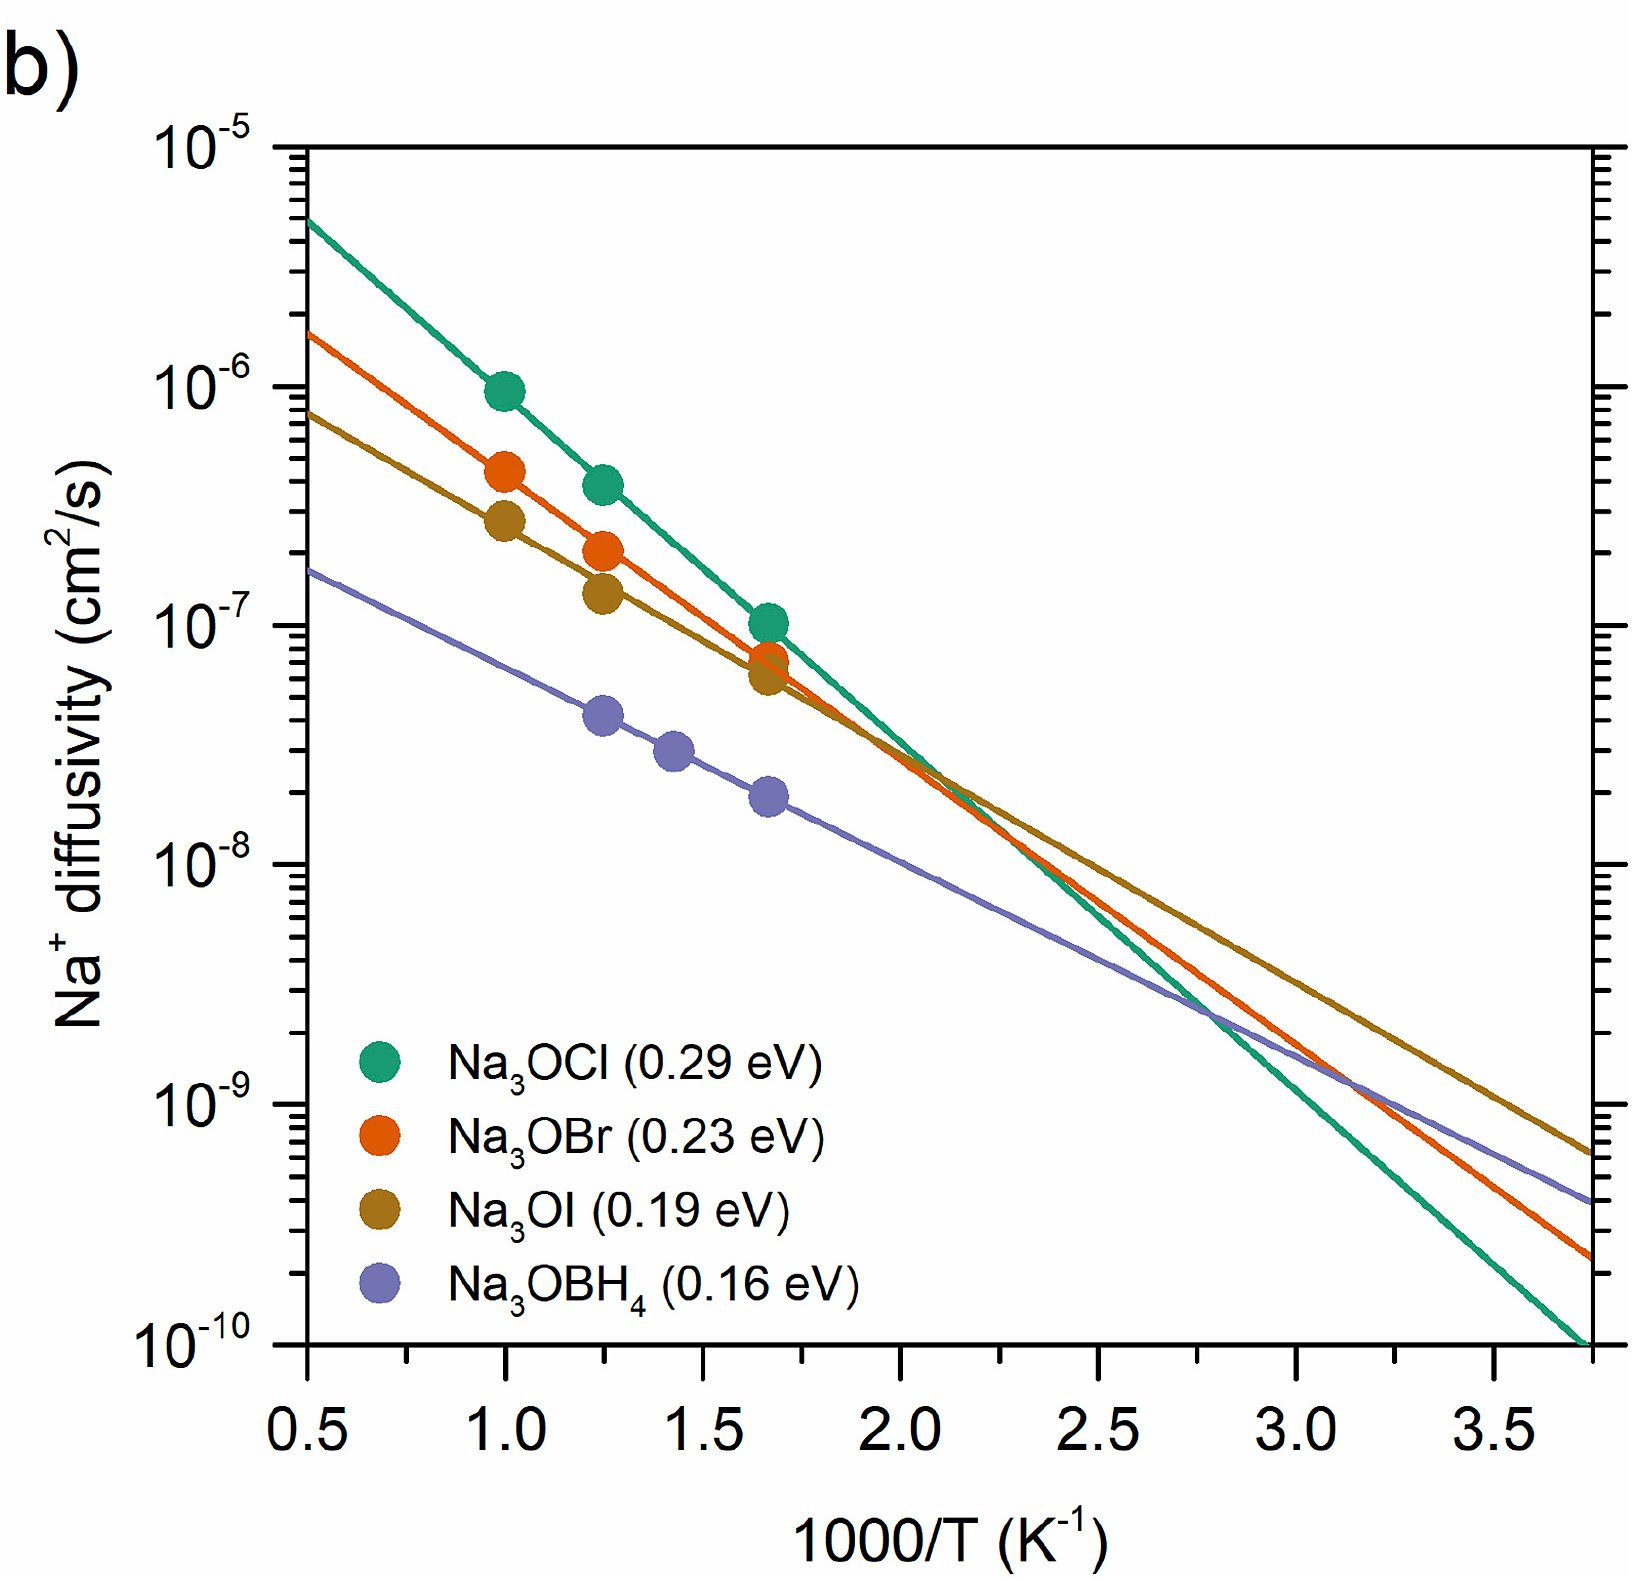
\includegraphics[width=7cm]{Ahiavi2020_calculated.jpg}
\end{figure}

\subsection{Conclusions}

\begin{itemize}
  \item Shown synthetic route without annealing
  \item Halogen size controls the lattice volume and implicitly the Na-ion conductivity of these materials
  \item The polarizability of the (super)halogen controls the activation energy for conduction through its effect on the lattice softness
  \item \ch{Na3OBH4} is not a positive outlier in terms of its ion transport
\end{itemize}

\section{Gao et al. (2020): Mechanism of enhanced ionic conductivity by
rotational nitrite group in antiperovskite \ch{Na3ONO2}}

\subsection{Methods}

\begin{itemize}
  \item Synthesis via grinding and sintering
  \item Powder X-ray diffraction
  \item Neutron powder diffraction
  \item Differential scanning calorimetry
  \item Electrochemical impedance spectroscopy
  \item Rietveld Refinements and maximum entropy method
analysis
  \item DFT via VASP with projector-augmented wave (PAW) method and PBEsol GGA with 2x2x1 supercell
\end{itemize}

\subsection{Synthesis and structure}

\begin{itemize}
  \item \ch{Na3ONO2} was found with antiperovskite structure
  \item \ch{Na3ONO3} was not possible, as the structure formed was not antiperovskite (tolerance factor)
\end{itemize}

\subsection{Experimental onductivity}

\begin{figure}[H]
\centering
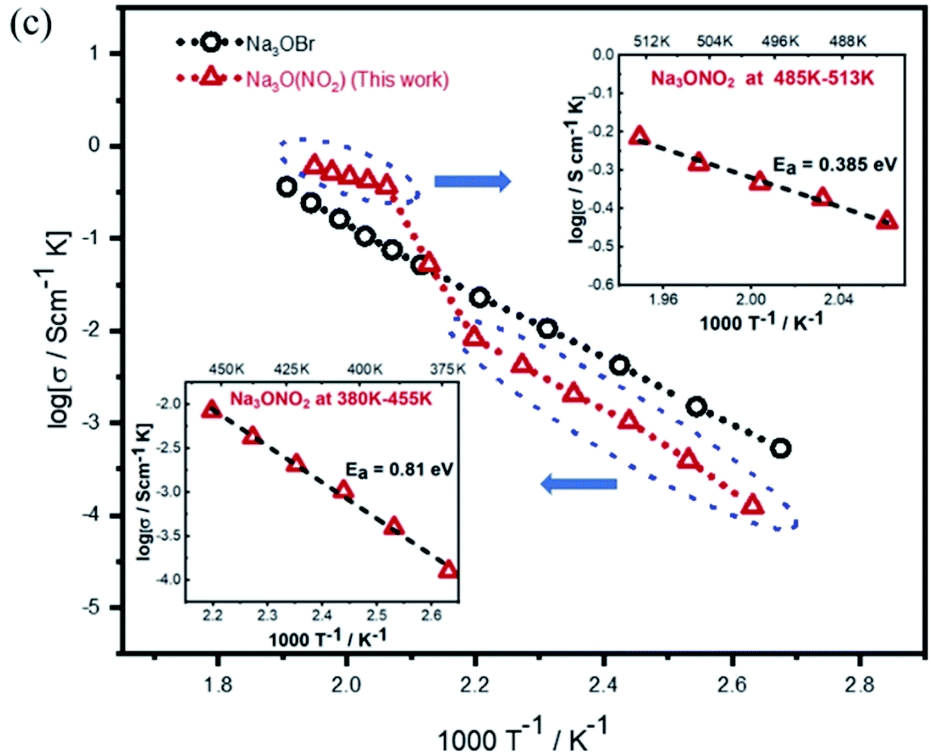
\includegraphics[width=7cm]{Gao2020_experimental.jpg}
\end{figure}

\subsection{Calculated conductivity}

\begin{itemize}
 \item DFT calculations reveal that the increased conductivity at higher temperatures is due to the rotation of the \ch{NO2} group
 \item According to calculations, the activation energy at these high temperatures drops to 0.37 eV (lower than \ch{Na3OBr})
\end{itemize}

\subsection{Conclusions}

\begin{itemize}
  \item At high temperatures, the rotation of the \ch{NO2} group leads to a lowered migration barrier and a higher conductivity via Na-O interactions
  \item Other anion clusters could show similar effects
\end{itemize}

\section{Li et al. (2020): Theoretical study of \ch{Na+} transport in the solid-state electrolyte \ch{Na3OBr} based on deep potential molecular dynamics}

\subsection{Methods}

\begin{itemize}
  \item Deep potential molecular dynamics (DeePMD) with LAMMPS
  \item Training potential from VASP with PAW and PBEsol functional
\end{itemize}

\subsection{Calculated conductivity}

\begin{figure}[H]
\centering
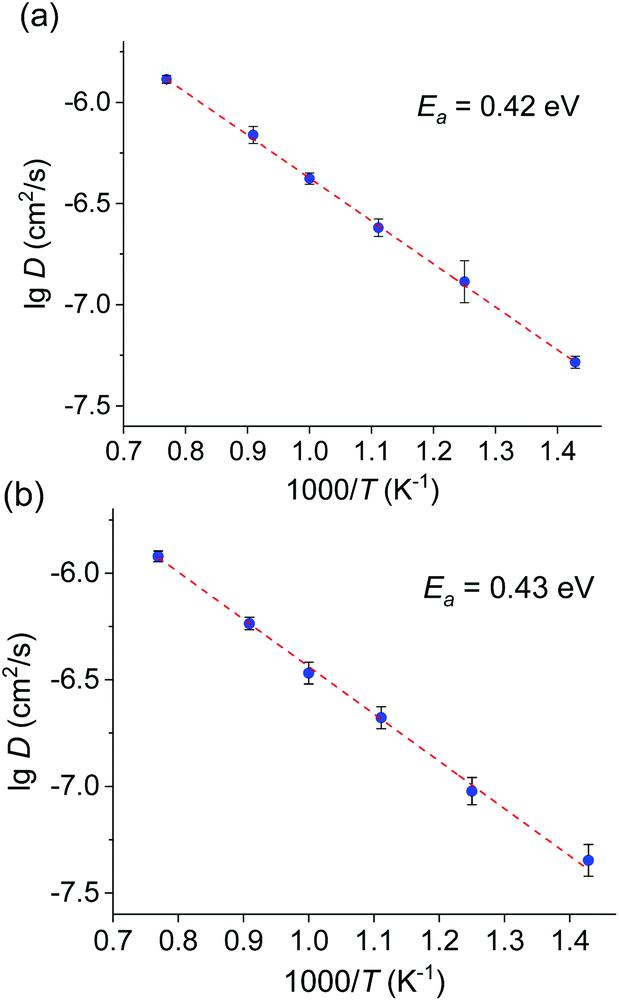
\includegraphics[width=7cm]{Li2020_conductivity.jpeg}
\end{figure}

\subsection{Conclusions}

\begin{itemize}
  \item Using the DP-based molecular dynamics technique, we have calculated the diffusion coefficient of Na3OBr in a temperature range of 700–1300 K
  \item Activation energy of 0.42-0.43 eV, which is rather close to the NEB migration barrier (0.41-0.43 eV)
  \item The extrapolated RT ionic conductivity at the experimental lattice parameter and vacancy concentration is estimated as $1 \times 10^{-4} - 2 \times 10^{-4} \, mS \, cm^{-1}$, in the same order of magnitude as the experimental results
\end{itemize}

\section{Fan et al. (2020): A Na-rich fluorinated sulfate anti-perovskite with dual doping as solid electrolyte for Na metal solid state batteries}

\subsection{Methods}

\begin{itemize}
  \item Synthesis with ball milling with the help of alcohol, followed by sintering
  \item Electrochemical impedance spectroscopy
\end{itemize}

\subsection{Experimental conductivity}

\begin{figure}[H]
\centering
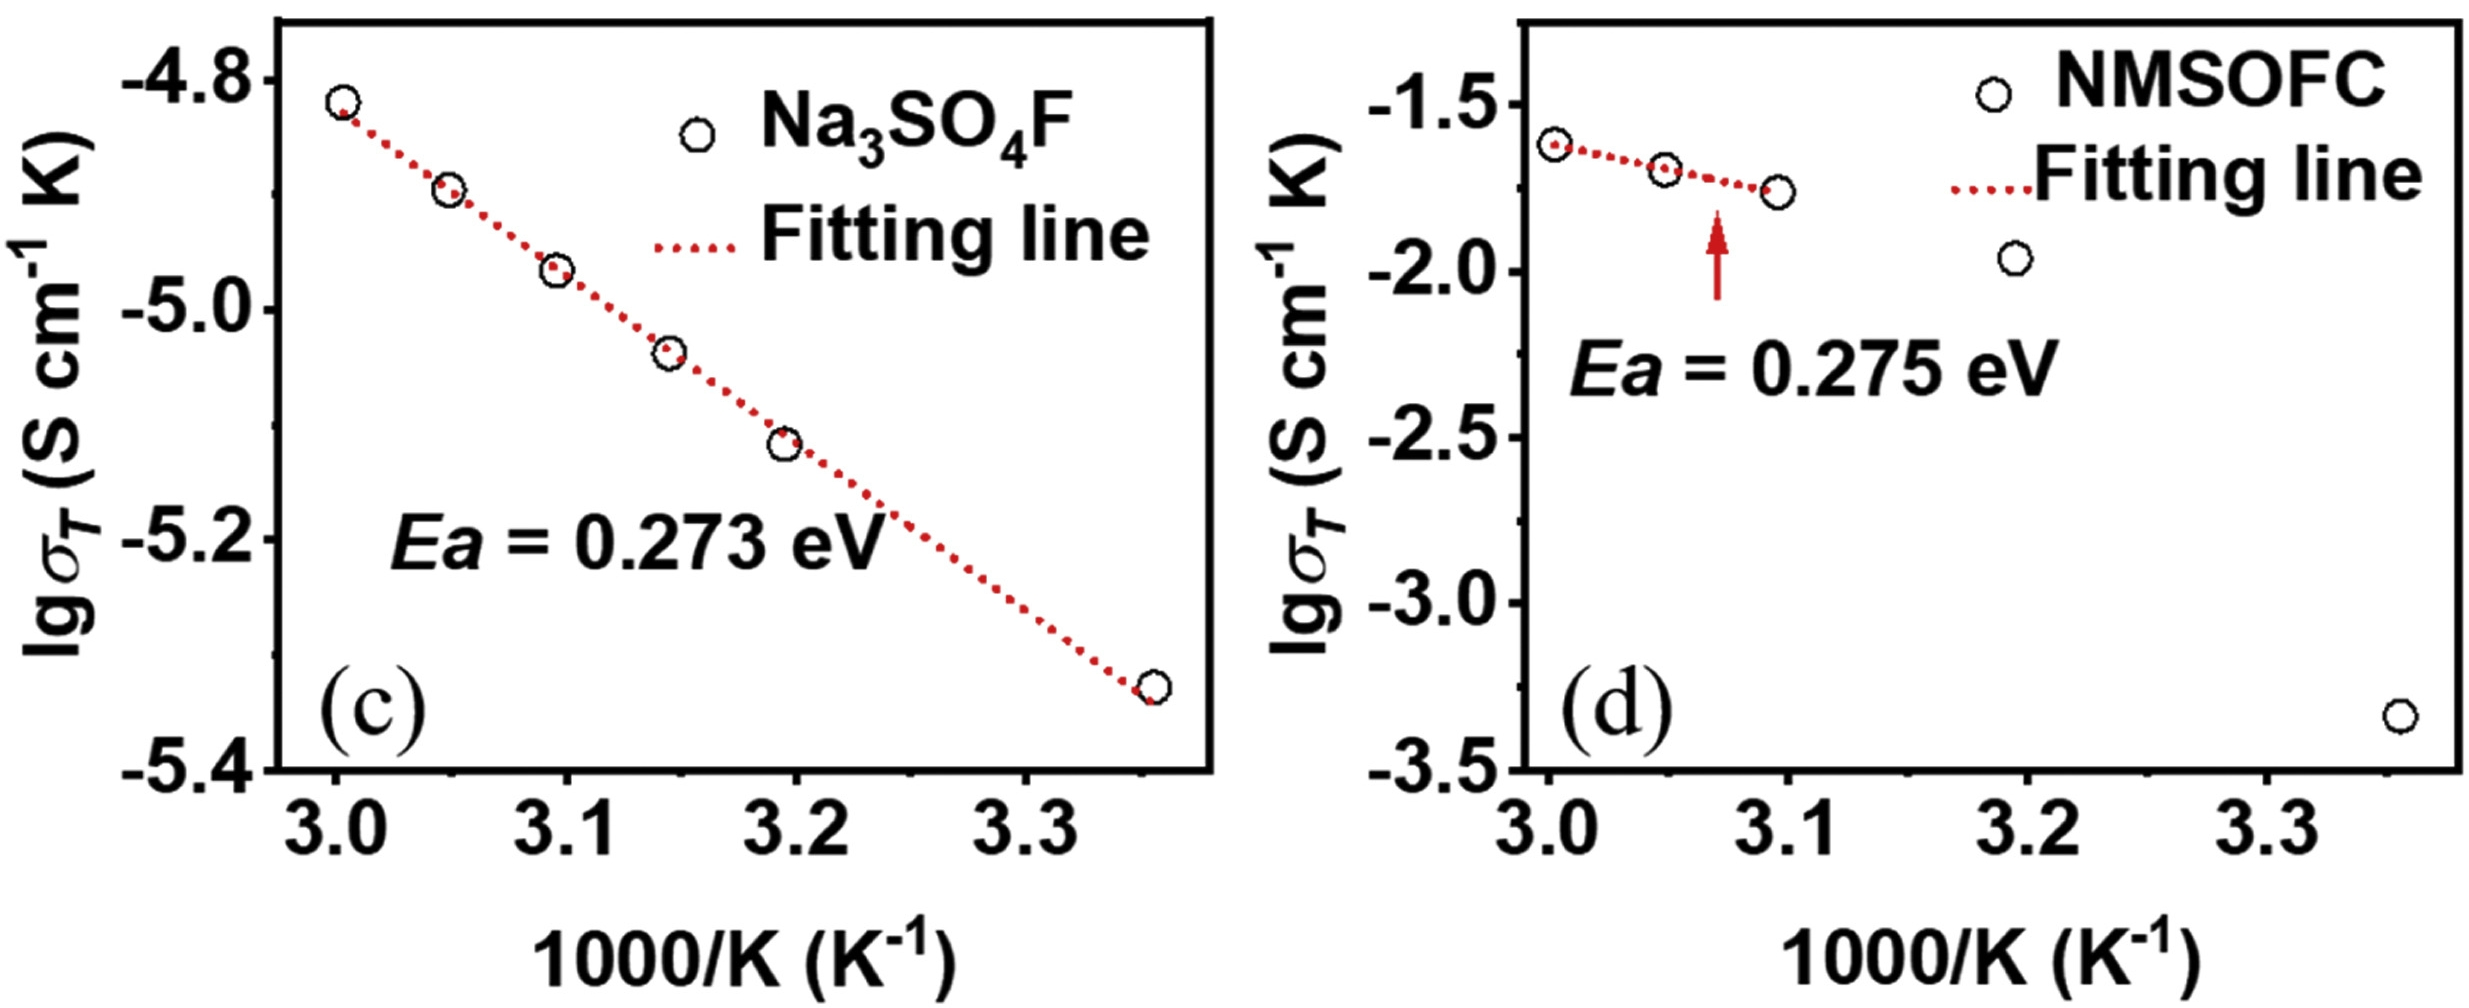
\includegraphics[width=7cm]{Fan2020_conductivity.jpg}
\end{figure}

\begin{itemize}
  \item \ch{Na_{2.98}Mg_{0.01}SO4F_{0.95}Cl_{0.05}} is denoted as NMSOFC
\end{itemize}

\subsection{Conclusions}

\begin{itemize}
  \item Na-rich fluorinated sulfate family with anti-perovskite structure is promising as high-conductivity Na-ion solid electrolyte by further doping and synthesis optimization
\end{itemize}

\section{Feng et al. (2020): Facile synthesis and electrochemical properties of Na-rich
anti-perovskite solid electrolytes}

\subsection{Methods}

\begin{itemize}
  \item Synthesis via solid state reaction with sintering from fresh made \ch{Na2O}
  \item X-ray diffraction
  \item Impedance spectroscopy
  \item $^{23}$Na NMR
\end{itemize}

\subsection{Experimental conductivity}

\begin{figure}[H]
\centering
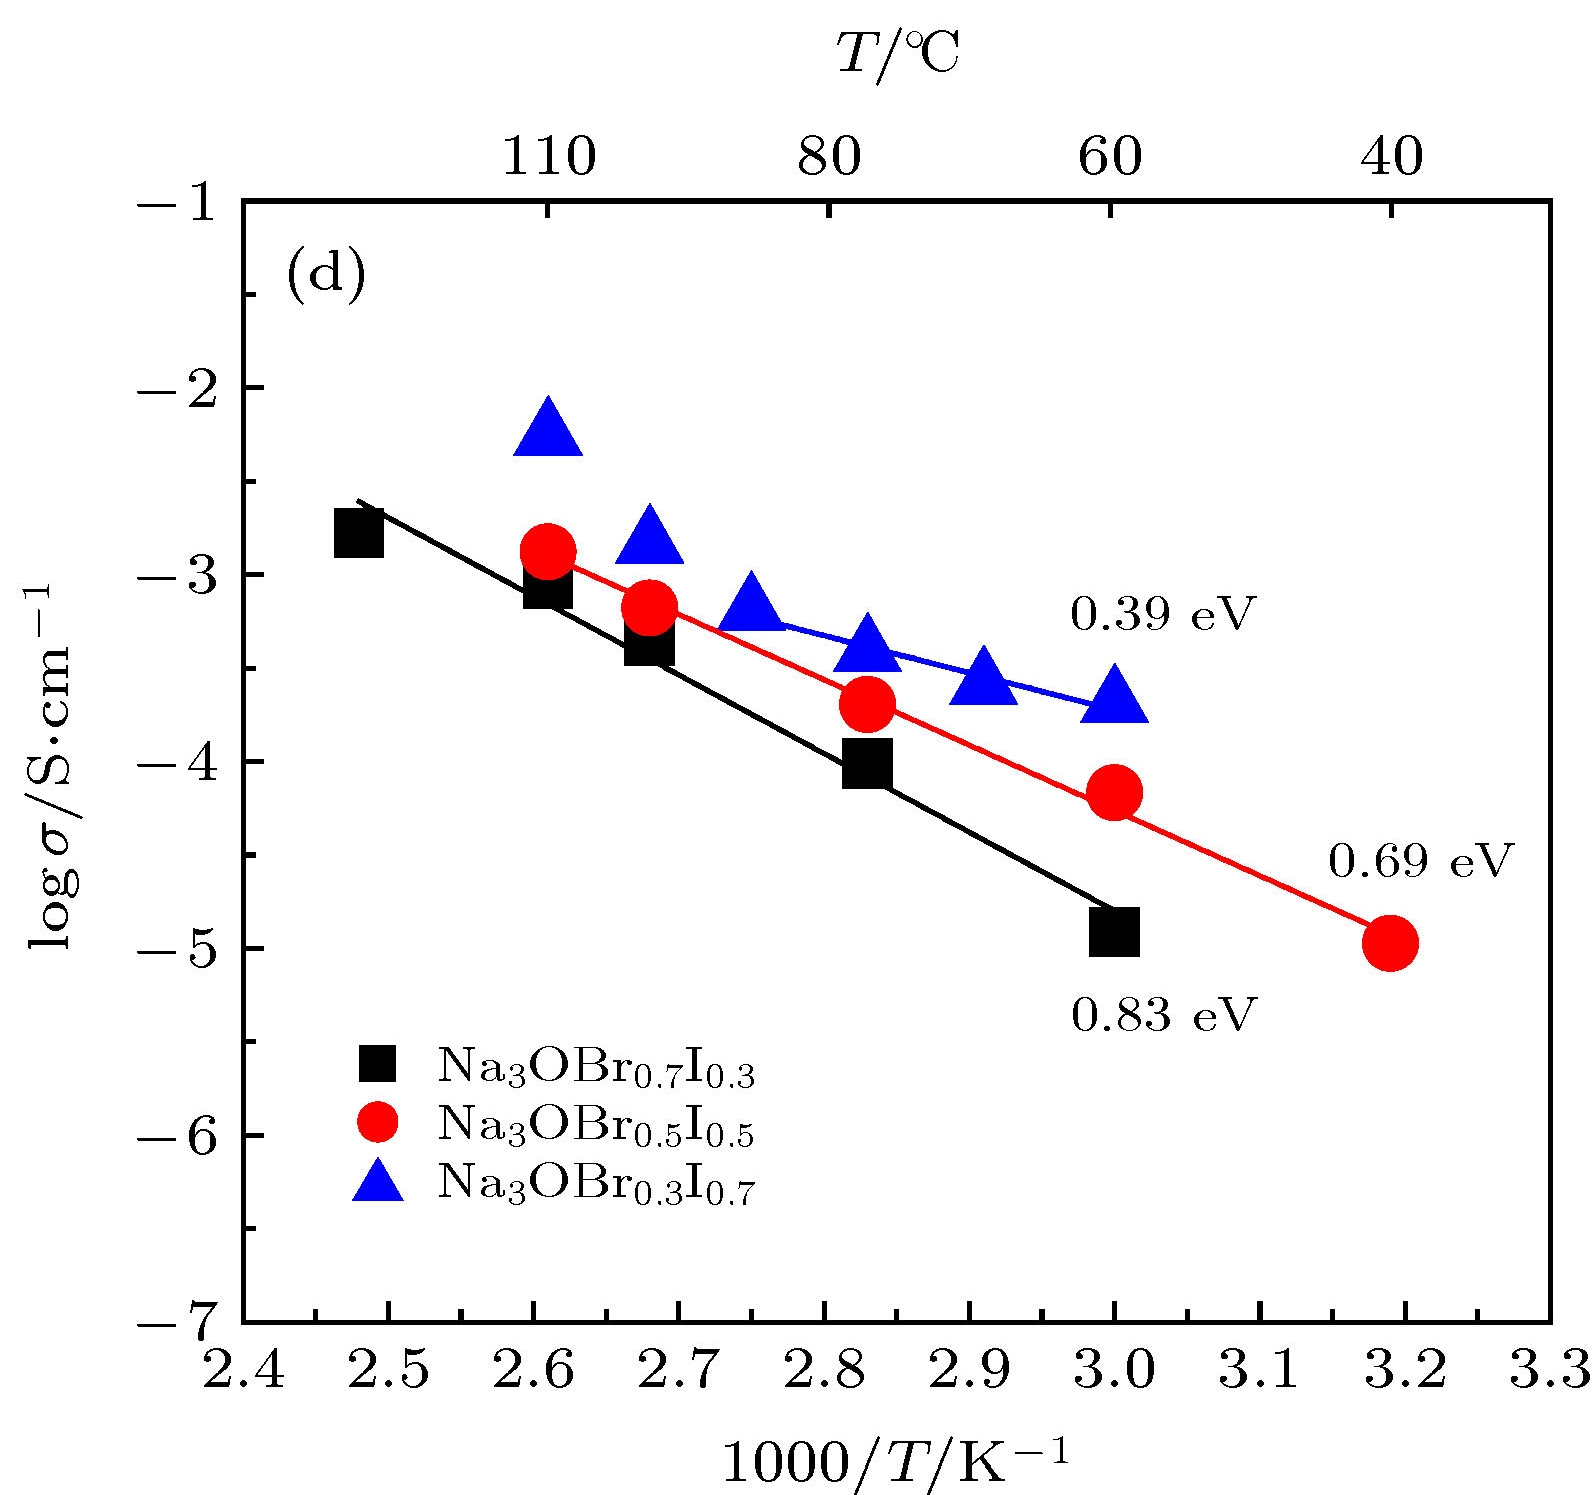
\includegraphics[width=7cm]{Feng2020_conductivity.jpg}
\end{figure}

\subsection{Conclusions}

\begin{itemize}
  \item Successful synthesis via simple single-step synthesis with heating to 373 K
  \item Conductivity in the range of $10^{-3} S/cm$ at around 373 K
\end{itemize}

\part{Papers on Structural Properties}

\section{Sabrowski et al. (1988): \ch{Na3OCl} and \ch{Na3OBr} the first alkali metal chalcogenide halides}

\subsection{Methods}

\begin{itemize}
  \item Synthesis via sintering
  \item Powder X-ray diffraction
\end{itemize}

\subsection{Synthesis and structure}

\begin{itemize}
  \item \ch{Na3OCl} lattice parameter: 4.500 $\AA$
  \item Also some elastic properties
\end{itemize}

\section{Hippler et al. (1990): Structure of \ch{Na3OCl}}

\subsection{Methods}

\begin{itemize}
  \item Synthesis via sintering
  \item Powder X-ray diffraction
\end{itemize}

\subsection{Synthesis and structure}

\begin{itemize}
  \item \ch{Na3OCl} lattice parameter: 4.496 $\AA$
\end{itemize}

\section{Zienko et al. (2001): Lattice Dynamics of Antiperovskite Structure
Compounds \ch{A3OX} (A = Na, K; X = CI, Br)}

\subsection{Methods}

\begin{itemize}
  \item DFT with LAPW and ab initio pseudopotentials
\end{itemize}

\subsection{Structure}

\begin{itemize}
  \item Lattice parameter for \ch{Na3OCl}: 4.31, \ch{Na3OBr}: 4.36
\end{itemize}

\subsection{Elastic and phonon properties}

\begin{itemize}
  \item Elastic constants
  \item Dielectric constants for \ch{Na3OCl}: 2.11, \ch{Na3OBr}: 2.20
\end{itemize}

\section{Ramanna et al. (2013): Ab initio study of electronic structure, elastic and optical properties of anti-perovskite type alkali metal oxyhalides}

\subsection{Methods}

\begin{itemize}
  \item DFT via CASTEP with plane wave pseudo-potential (PW-PP) method and via Wien2K with full potential linearized augmented plane wave (FPLAPW) method
  \item Both GGA and LDA calculations were performed
\end{itemize}

\subsection{Structure}

\begin{itemize}
  \item A range of lattice parameters found for \ch{Na3OCl} and \ch{Na3OBr}
\end{itemize}

\subsection{Elastic and phonon properties}

\begin{itemize}
  \item Bulk, shear, Young's, Poisson's, anisotropy factor and Cauchy's pressure for \ch{Na3OCl} and \ch{Na3OBr}
  \item Dielectric constants for \ch{Na3OCl}: 1.97, \ch{Na3OBr}: 2.22
\end{itemize}

\section{Wang el at. (2016): Robust high pressure stability and negative thermal expansion in sodium-rich antiperovskites \ch{Na3OBr} and \ch{Na4OI2}}

\subsection{Methods}

\begin{itemize}
  \item Synthesis via solid-state method
  \item High pressure angle-dispersive XRD
  \item DFT via CASTEP and LDA
\end{itemize}

\subsection{Synthesis and structure}

\begin{itemize}
  \item Antiperovskite and layered antiperovskite structures confirmed
  \item Both stable up to 24.3 GPa pressure
\end{itemize}

\subsection{Thermal data}

\begin{itemize}
  \item Negative thermal expansion at lower temperatures 20-80K
  \item The phase stability was further explored with the DFT calculations
\end{itemize}

\section{Deng et al. (2016): Elastic Properties of Alkali Superionic Conductor Electrolytes
from First Principles Calculations}

\subsection{Methods}

\begin{itemize}
  \item Used VASP code to run DFT calculations with the projector augmented wave (PAW) method and generalised gradient approxiamtion (GGA)
\end{itemize}

\subsection{Elastic properties}

\begin{itemize}
  \item Bulk, shear, Young's, Poisson's, Pough's found for \ch{Na3OCl} and \ch{Na3OBr}
\end{itemize}

\section{Lv et al. (2017): Electronic, elastic, lattice dynamic and thermal conductivity properties of \ch{Na3OBr} via first principles}

\subsection{Methods}

\begin{itemize}
  \item DFT via CASTEP with GGA-PBESOL functional
\end{itemize}

\subsection{Strcuture}

\begin{itemize}
  \item \ch{Na3OBr} lattice constant: 4.5729 $\AA$
  \item Band gap of 1.81 eV
\end{itemize}

\subsection{Elastic and phonon properties}

\begin{itemize}
  \item Bulk, shear, Young's, Poisson's, Pough's found 
  \item At 300 K,the predicted thermal conductivity is about $7.30 W m^{-1}K^{-1}$
  \item Dielectric 3.23
  \item Static dielectric: 10.09
\end{itemize}

\section{Pham et al. (2018): Computational predictions of stable phase for antiperovskite \ch{Na3OCl} via tilting of \ch{Na6O} octahedra}

\subsection{Methods}

\begin{itemize}
  \item Used VASP code to run DFT calculations with the projector augmented wave (PAW) method and generalised gradient approxiamtion (GGA) and local density approximation (LDA)
  \item Structures used are either 6x6x6 or 8x8x8 supercells
\end{itemize}

\subsection{Structure}

\begin{itemize}
  \item \ch{Na3OCl} lattice parameter: 4.538 $\AA$ (GGA) or 4.382 $\AA$ (LDA)
  \item Band gap for cubic phase: 3.4 eV
  \item Formation energy: -72.7 meV/formula unit
\end{itemize}

\subsection{Phase stability conclusions}

\begin{itemize}
  \item Investigated whether tilting of the \ch{Na6O} octahedral leads to increased stability
  \item 14 tilted structures of Na3OCl were energetically more stable than the cubic $Pm\overline{3}m$ structure, and the $P2_{1}/m$ phase is energetically the most stable one
  \item Found that the cubic $Pm\overline{3}m$ phase has a direct band gap of 3.4 eV at the Gamma point, and the monoclinic $P2_{1}/m$ phase has a quite similar result (3.38 eV), which indicates that the material is insulating
\end{itemize}

\section{Khandy et al. (2020): Electronic structure, thermomechanical and phonon properties of inverse perovskite oxide (\ch{Na3OCl}): An ab initio study}

\subsection{Methods}

\begin{itemize}
  \item DFT via Wien2K with full potential linearized augmented planewavve (FPLAPW) and GGA
\end{itemize}

\subsection{Structure}

\begin{itemize}
  \item \ch{Na3OCl} lattice parameter: 4.53 $\AA$
  \item Band gap of 2.18 eV (higher than that of \ch{Na3OBr}, which was 1.18 eV)
\end{itemize}

\subsection{Elastic and phonon properties}

\begin{itemize}
  \item Bulk, shear, Young's, Poisson's, Pough's and anisotropy factor calculated
  \item Lattice thermal conductivity: \ch{Na3OCl} has 6.48 W/mK is comparable to \ch{Na3OBr} 7.30 W/mK
  \item Maximum magnetic susceptibility was  about $9 \times 10^{12} \, emu/mol$ at 50 K
\end{itemize}

\section{Sattar et al. (2020): The structural stability, lattice dynamics, electronic, thermophysical, and mechanical properties of the inverse perovskites \ch{A3OX}: A comparative first‐principles study}

\subsection{Methods}

\begin{itemize}
  \item DFT via Wien2K and full potential linearized augmented wave (FP‐LAPW) method with GGA on 2x2x2 supercell
\end{itemize}

\subsection{Structure}

\begin{itemize}
  \item Lattice parameters: \ch{Na3OCl}: 4.541 $\AA$, \ch{Na3OBr}: 4.631 $\AA$, \ch{Na3OI} 4.740 $\AA$
  \item Band gaps:\ch{Na3OCl}: 2.204 eV, \ch{Na3OBr}: 1.872 eV, \ch{Na3OI} 1.977 eV
\end{itemize}

\subsection{Elastic and phonon properties}

\begin{itemize}
  \item Elastic constants, bulk, shear, Cauchy pressure, Poisson's, Young's, Pugh's, and anisotropic factor, Vickers hardness, Hardness, transverse and longitudinal elastic wave velocity, average wave velocity and Debye temperature 
  \item Electronic conductivity, electronic and lattice thermal conductivity
  \item Vibrational modes
\end{itemize}

\part{NMR-related Papers}

\section{Klosters et al. (2000): Determination of the (\ch{Na+}) Sternheimer antishielding factor by Na-23 NMR spectroscopy on sodium oxide chloride, \ch{Na3OCl}}

\section{Johnson et al. (2005): Periodic ab initio calculation of nuclear quadrupole parameters as an assignment tool in solid-state NMR spectroscopy: applications to Na-23 NMR spectra of crystalline materials}

\end{document}